% % CHAPITRE 1 : SYNTHESE BIBLIO
%
%Réflexions
%
%NE PAS OUBLIER DE CALER UN MAXIMUM D'ORDRE DE GRANDEUR ! 
%	(émissions CO2, CH4, stocks flux, surface des tourbières, végétation ...)
%
%Bien différencier l'intro générale qui doit être lisible par un béotien, de l'intro au travail de la thèse qui doit être un état de l'art précis et documenté sur les travaux antérieurs (synthèse biblio)
%
%Ou caler la partie de biblio sur l'expérimentation ... (peut être dans la synthèse biblio, paragraphe "approche mise en oeuvre"
%INTRODUCTION GENERALE (à mettre dans le chapitre Intro)
%
%- Qu'est ce qu'une tourbière ? (Éventuellememt comment se forme-t-elle ?)
%	*Définition
%	*Formation/Évolution (stockage du C, battement de la nappe ?)
%	*Classification
%- Les tourbières et les hommes 
%	*Usages d'hier et d'aujourd'hui (Combustible, horticulture, matériau de construction)
%	*Les thématiques scientifiques (pourquoi les avoir étudier et les étudier en gros)
%	*Le contexte dans lequel va s'inscrire le travail qui suit
%
%SYNTHESE BIBLIOGRAPHIQUE
%
%- Quelles sont les grandes thématiques de recherche liées aux tourbières ?
%	*Exploitation
%	*Archives
%	*Émissions de GES
%- Plus précisément quelles sont les grands axes de recherche sur ces écosystèmes et liés aux émissions de GES.
%	*Processus de création de GES (CO2 et CH4) (Facteurs contrôlant généralement invoqués)
%	*Processus de migration des GES dans le profil
%	*Processus de stockage/capture
%- Approches mise en oeuvre
%	*Modélisation (empirique et mécaniste)
%	*Expérimentation (différentes techniques pour mesurer les émissions de GES, différentes techniques de chambre...)
%	*Variabilité spatio-temporelle (notion d'échelle)
%	
%	DOIS-JE TRAITER
%	La classification des tourbières ?
%	Hummock and Hollow ? Dire qu'on n'est pas dans ce niveau de détail ?
%	
%
%HISTORIQUE (études concernant les tourbières)
%
%1968-1969  Boelter : propriétés physique des tourbes
%1977 Boelter : hydrologie, caractéristique des sols organiques, chimie des écoulements
%1978 Ingram : Classification
%1981 Parkinson : Déjà l'amélioration d'une méthode pour la mesure des émissions de la respiration du sol
%1984 Clymo : Les limites à la croissance des tourbières
%1986 Chason : Conductivités hydraulique et propriétés physiques
%1989 Moore : Influence du niveau de la nappe sur les émissions de CO2 et de CH4
%//1990 Raich : Comparaison de 2 méthodes de chambre statique pour mesurer les flux de CO2
%1991 Gorham : Rôle des tourbières dans le cycle du carbon et réponse au changement climatique
%//1992 Raich : Flux de CO2 dans la respiration du sol et relation vis à vis du climat et de la végétation
%1992 Roulet : Flux de méthane (fen) et changement climatique
%1993 Bubier : Émission de méthane dans les zones humides
%1993 Bubier : Microtopographie et flux de méthane dans tourbières boréales.
%1993 Abbès : Sorption de l'ammonium ? (ammonia) par la tourbe et fractionnement de l'azote
%1994 Lloyd : Dépendance de la respiration du sol à la température
%1994 Bubier : Perspective écologique sur les émissions de méthane dans les zones humide de l'hémisphère nord
%//1994 Nay : Biais des méthodes de chambre pour la mesure des flux de CO2
%1995 Kirschbaum : Dépendance à la température de la décomposition de la MO (effet sur stock de C et changement Clim)
%1995 Bubier : Prédiction des émissions de méthane à partir de la distribution des bryophytes (tourbière hémisphère nord)
%1995 Bubier : Contrôles "écologique" sur les émissions de méthane dans les tourbières de l'hémisphère nord
%1995 Bubier : Relation entre la végétation avec les émissions de méthane et les gradients hydrochimique
%//1995 Bekku : Mesure de la respiration du sol avec une méthode de chambre fermée (IRGA)

% PLAN (2015-03-03)
%I. Définitions
%1 Tourbières/Tourbe (surface, type, localisation, biodiversité, services écologiques...)
%2 Classification
%3 Historique
%	a Utilisation
%	b Études scientifiques
%	
%Transition : Réaction aux changements globaux (comment fonctionnent-elles ?)
%
%II. Fonctionnement
%1 Stock
%2 Flux
%	a Entrants (Photosynthèse)
%	b Sortants (Méthanogénèse, Respiration)
%3 Facteurs Contrôlant
%	a Hydrologie (WTL,HR)
%	b Propriétés physiques (T, densités, conductivités thermiques...)
%	c Végétation (Bryophytes/Vasculaires)
%	d Météo

% GO TO intro générale ?
%Depuis quand sont-elles étudiées ?
%D'abord étudiées pour leurs propriétés physiques afin de connaitre leur qualité en tant que combustible.
%Elle sont maintenant majoritairement étudiée à travers le prisme des changements globaux.
%Ainsi les études concernent les flux de GES, ...
\singlespacing
\chapter{Synth\`{e}se bibliographique}
\label{ch:ch1}

\minitoc

\newpage
\doublespacing
\index{tourbières|(}
%Dans ce chapitre, nous commenceront par donner une vue de ce que sont les tourbières : Que sont-elles ? Depuis quand sont-elles étudiées ? Pourquoi les a-t-on étudiés ?
%Nous continuerons en entrant plus en détails sur leur fonctionnement vis à vis des flux de carbone.
%Enfin nous verrons quels sont les facteurs contrôlant majeurs de ces flux.
La première partie de ce chapitre traite des tourbières de façon générale : Que sont ces écosystèmes ?
Quelle terminologie y est associée ? Comment se forment-ils ? Quelle est leur situation dans le monde d'aujourd'hui ?
La seconde partie décrit plus spécifiquement les tourbières à travers le prisme des flux de carbone, principalement gazeux : 
Quel sont les liens entre la structure et le fonctionnement des tourbières et les flux de carbone ? 
Quels sont les facteurs qui contrôlent ces flux ? 
Quels est l'état des connaissances quant à l'estimation des bilans de carbone dans ces écosystèmes ?

\section{Les tourbières et le cycle du carbone}

Que se soit dans leurs définitions ou leurs modes de formation, les tourbières sont des écosystèmes indissociables du cycle du carbone.

\subsection{Zones humides et tourbières : définitions et terminologies}

\subsubsection{Définitions}

Les tourbières font partie d'un ensemble d'écosystèmes plus large que l'on appelle les zones humides\index{zone humide} (\textit{wetlands}).
Ces zones humides ne sont ni des écosystèmes terrestres au sens strict, ni des écosystèmes aquatiques.
Elles sont à la frontière entre ces deux mondes et sont caractérisées par un niveau de nappe élevé, proche de la surface du sol, voire au dessus.
Cette omniprésence de l'eau joue fortement sur l'aération du sol et contraint, de façon plus ou moins importante, l'accès à l'oxygène.
Les zones humides ont été définies en 1971, lors de la convention de \textsc{Ramsar}\footnote{La convention de \textsc{ramsar} est un traité international visant à la conservation et l’utilisation rationnelle des zones humides.} de la façon suivante : 
\begin{pdef}
\textsc{Zone humide} :

«les zones humides sont des étendues de marais, de fagnes\footnotemark, de tourbières ou d'eaux naturelles ou artificielles, permanentes ou temporaires, où l'eau est stagnante ou courante, douce, saumâtre ou salée, y compris des étendues d'eau marine dont la profondeur à marée basse n'excède pas six mètres.»

\hfill {\scriptsize \citep{ramsar1987}}
\end{pdef}
\footnotetext{Marais tourbeux situé sur une hauteur}

Les zones humides regroupent donc des écosystèmes très variés parmi lesquels les marais, les mangroves, les plaines d'inondations et les tourbières.
Ces dernières sont des écosystèmes majoritairement continentaux (par opposition aux écosystèmes côtiers comme les deltas) et ont comme particularité d'avoir, comme toutes les zones humides, un niveau de nappe élevé et donc une zone anaérobie importante.
Ceci induit le développement de communautés microbiennes et végétales spécifiques, adaptées aux milieux humides ou inondés.
Les sphaignes sont caractéristiques de ces écosystèmes, ce sont des mousses, des bryophytes\footnote{Les bryophytes sont des végétaux caractérisés par un système vasculaire absent. Ces plantes n'ont pas de racines mais des rhizoïdes.} de la famille des \textit{Sphagnaceae}.
%Leurs particularités : niveau de nappe élevé et zone anaérobie importante, entraînent le développement d'une végétation spécifique, qui s'est adaptée aux milieux fortement humides ou inondés.

Les tourbières représentent 50 à \SI{70}{\percent} des zones humides \cite{joosten2002}.
Leur définition est variable selon les régions (\plop, exple).
%Cela ne facilite pas leur recensement et leur cartographie.
Deux définitions sont régulièrement utilisées :

\begin{pdef}
\textsc{Tourbière} :

Écosystème, avec ou sans végétation, possédant au moins \SI{30}{\cm} de tourbe naturellement accumulée.

\hfill {\scriptsize Définition traduite d'après \citet{joosten2002}}
\end{pdef}
%La première définie comme tourbières les écosystèmes possédant au moins \SI{30}{\cm} de tourbe (parfois 40).
Cette première définition correspond au \textit{peatland} anglo-saxon.
L'épaisseur de tourbe accolée à cette définition peut varier selon le pays, elle est par exemple établie à \SI{40}{\cm} au Canada \citep{nationalwetlandsworkinggroup1997}.
Une autre définition existe :

\begin{pdef}
\textsc{Tourbière active} :

Écosystème dans lequel un processus de tourbification est actif.

\hfill {\scriptsize Définition traduite d'après \citet{joosten2002}}
\end{pdef}
Cette seconde définition correspond au \textit{mire} anglo-saxon et peut être traduite en français par le terme de tourbière active.
Les concepts derrière ces deux définitions se chevauchent mais ne sont pas complètement similaires : une tourbière drainée peut, par exemple, avoir plus de \SI{30}{cm} de tourbe et ne plus former de tourbe, ne plus être active.
À l'inverse il peut exister des zones où l'épaisseur de tourbe est inférieure à \SI{30}{cm} malgré un processus de tourbification actif.
Un même écosystème tourbeux peut d'ailleurs contenir à la fois des zones qui correspondent à la première définition et d'autres à la seconde.
%Elles sont généralement définies par rapport à la tourbe, qu'il convient donc de définir au préalable.
%La tourbe est un sol organique (histosol) formé suite à l'accumulation de litières végétales partiellement décomposées dans un milieux saturé en eau.
Les tourbières sont donc, selon la définition utilisée, des écosystèmes contenant ou des écosystèmes formant de la tourbe.
Mais qu'est ce que la tourbe ?

\begin{pdef}
\textsc{Tourbe} :

«Accumulation sédentaire\footnotemark de matériel composé d'au moins \SI{30}{\percent} (matière sèche) de matières organiques mortes.»

\hfill {\scriptsize Définition traduite d'après \citet{joosten2002}}
\end{pdef}
\footnotetext{\citet{joosten2002} distinguent sédimentaire de sédentaire dans le sens où dans le premier cas la matière migre (dans la colonne d'eau par exemple) entre la zone où elle est produite et la zone où elle est stockée, ce qui n'est pas le cas pour le second cas où ces zones sont confondues.}

Le seuil de \SI{30}{\percent} est souvent utilisé pour rapprocher sa définition de celle d'un sol organique (histosol) au sens large, dans lesquels sont classés la majorité des sols tourbeux (selon la classification).
D'autres définitions existent, faisant la distinction entre sols organiques et tourbes avec un seuil à \SI{75}{\percent} \citep{andrejko1983} ou \SI{80}{\percent} \citep{landva1983}.
Il est également nécessaire de préciser qu'au delà de la classification utilisée ce que les écologues considèrent comme de la tourbe contient généralement \SI{80}{\percent} de matières organiques au minimum \citep{rydin2013b}.
Ce processus de formation est appelé la tourbification\index{tourbification} ou turfigénèse et les matières organiques accumulées proviennent majoritairement de la végétation.
On définit les matières organiques de la façon suivante : 
\begin{pdef}
\textsc{Matières organiques} :

Matières constituées d'un assemblage d'éléments ayant une ou plusieurs liaison C--H formant de nombreux composés organiques dont des carbohydrates (sucres, cellulose \dots), des composés azotés (protéines, acides aminés \dots) et phénoliques (lignine \dots), des lipides (cires, résines, \dots) et d'autres\footnotemark.

%\hfill {\scriptsize Définition traduite d'après \citet{joosten2002}}
\end{pdef}
\footnotetext{Cette définition, utile pour définir simplement les matières organiques, est cependant limitée car elle inclut des composés traditionnellement considérés comme minéraux (le graphite) et en exclut d'autres considérés comme organiques (acide oxalique) (Liste de diffusion ResMO (Réseau Matières Organiques \url{http://www6.inra.fr/reseau_matieres_organiques})).}

%La tourbe peut être considérée comme du charbon (?coal) dans ses stades les plus précoces. 
%En continuant à évoluer, à se compacter, se formerai  (combien de temps) d'abord de la lignite puis du charbon et enfin de l'anthracite (belanger 1988 dans Rydin et Jeglum 2006)
%Les propriétés physiques de la tourbe dépendent du type de végétation, mais également de sa profondeur dans le profil (pédogenèse, diagenèse) amha2010 dans rydin.

\subsubsection{Distribution des tourbières à l'échelle mondiale}

L'hétérogénéité des définitions ajoutées aux limites floues qui peuvent exister entre certains écosystèmes tourbeux et non-tourbeux rendent la cartographie de ces écosystèmes délicate.
Les estimations généralement citées évaluent la surface occupée par les tourbières à environ \SI{4000000}{\square\kilo\meter} \citep{lappalainen1996}.\index{tourbières!surface} 
Cette surface correspond à \num{2} à \SI{3}{\percent} de l'ensemble des terres émergées du globe.
Plus de \SI{85}{\percent} d'entre elles sont situées dans l'hémisphère nord, majoritairement dans les zones boréales et sub-boréales \citep{strack2008} (Figure~\ref{fig:peatlandGlobalDistribution}).
Ce travail sera focalisé sur ces écosystèmes, laissant de côté les tourbières tropicales dont le fonctionnement est distinct et spécifique \plop.

\begin{figure}
\centering
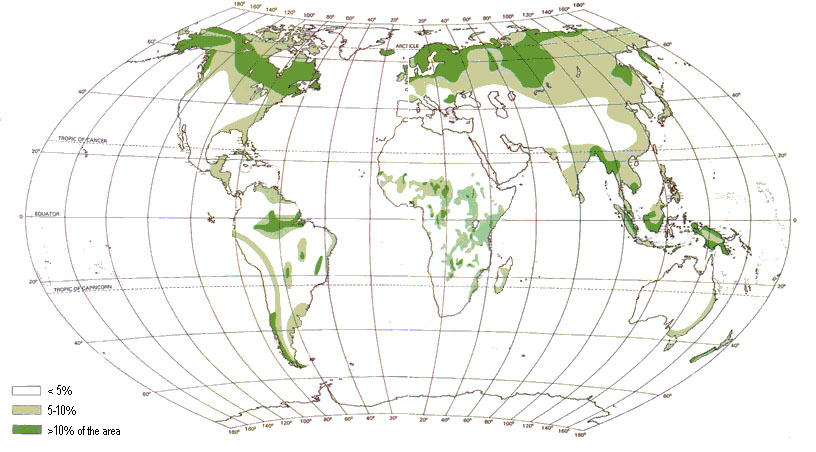
\includegraphics[width=\textwidth]{chap1/peatlandGlobalDistribution}
\caption{Distribution mondiale des tourbières en pourcentage de surface recouverte.}
\label{fig:peatlandGlobalDistribution}\index{tourbières!distribution} 
\end{figure}

\subsubsection{La formation des tourbières}

\begin{figure}
\centering
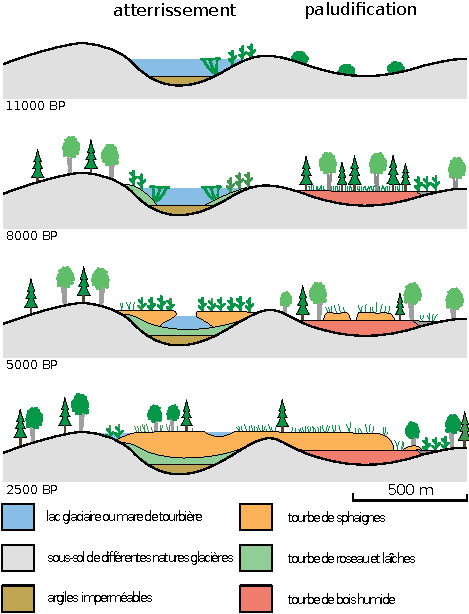
\includegraphics[width=\textwidth]{chap1/peat_formation}
\caption{Processus de formation des tourbières, à gauche l'atterrissement et à droite la paludification. Modifié d'après \citet{manneville1999}}
\label{fig:peat_formation}
\end{figure}

\index{tourbières!formation} 
L'atterrissement\index{atterrissement} et la paludification\index{paludification} sont les deux processus principaux permettant la formation des tourbières (Figure~\ref{fig:peat_formation}).
Il s'agit pour le premier du comblement progressif d'une zone d'eau stagnante (Figure~\ref{fig:peat_formation}).
Ce comblement est généralement lié à l'action combinée d'apports exogènes et d'une végétation colonisant les eaux en formant des tremblants\footnote{Radeau végétal, composé de végétation vivante et de débris qui peut masquer la surface de l'eau}.
La paludification est la formation de tourbe directement sur un sol minéral, grâce à des conditions d'humidité importante dans des zones peu perméables et topographiquement favorables (dépressions).
Ces modes de formation ne sont pas exclusifs, une tourbière pouvant se développer, selon les endroits considérés ou le temps, via des processus différents.

\subsubsection{Classifications}

Différentes classifications sont utilisées pour différencier ces écosystèmes.
La plus générale et la plus utilisée dans la littérature distingue les tourbières dite hautes, ou de haut-marais \textit{bog}, et les tourbières basses, ou de bas-marais \textit{fen}.

Les tourbières de haut-marais ont généralement une épaisseur de tourbe supérieure à \SI{30}{\cm} et sont alimentées principalement par les précipitations : elles sont dites ombrotrophes.
Leur surface parfois bombée (tourbières élevées ou bombées) peut également être plate ou en pente.
Cette géométrie situe une partie au moins de l'écosystème au dessus du niveau de la nappe.
Elles ont une concentration en nutriments relativement faible (oligotrophes) et renferment des eaux acides dont le pH est compris entre 3.5 et 4.2 \citep{rydin2013a}.

Les tourbières de bas-marais ont une épaisseur généralement supérieure à \SI{30}{\cm} avec un niveau de nappe très proche de la surface du sol.
De forme concave ou en pente, elles sont généralement alimentées en eau par des sources ou par ruissellement et sont donc dites minérotrophes.
Le pH de leur eaux de surface varie de 4 à 8.
Les végétations dominantes de ces écosystèmes peuvent être des bryophytes, des graminées ou des arbustes bas \citep{rydin2013a}.
%De nombreux critères existent pour classer les tourbières selon leur mode de formation, leur source d'eau, leur physico-chimie.
%La terminologie utilisée concernant ces écosystèmes n'a pas toujours été cohérente, de nombreux termes ont été utilisés parfois en contradiction les uns avec les autres \cite{joosten2002}.
%Il existe différents types de tourbières, notamment on distingue des tourbières tempérées/boréales des tourbières tropicales dont le fonctionnement diffère.
%Dans la suite de ce document seule les tourbières tempérées/boréales seront décrites et étudiées.

Au sein de ces écosystèmes la topographie est fortement variable et fait l'objet d'une terminologie particulière : on parle de buttes (\textit{hummock}) pour désigner des sur-élévation topographiques, de gouille (\textit{hollow}) pour les dépressions et de replat (\textit{lawn}) pour les zones entre les deux (Figure~\ref{fig:microtopo}).


\begin{figure}[t]
\centering
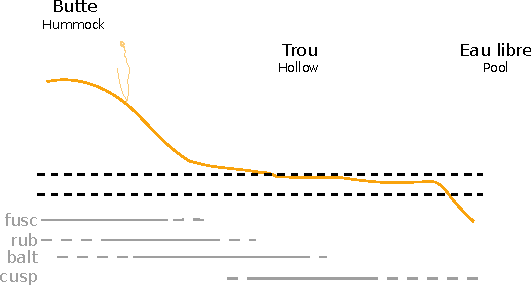
\includegraphics[width=\textwidth]{chap1/microtopo}
\caption{Micro-topographie dans les tourbières. Modifié d'après \citet{rydin2013a}}
\label{fig:microtopo}
\end{figure}

\subsection{Tourbières et fonctions environnementales}

%\subsubsection{Puits de carbone}
\subsubsection{Fonction puits de carbone}
\index{carbone!stock}
Par définition les tourbières stockent ou ont stocké du carbone.
Cette fonction puits de carbone rend ces écosystèmes importants vis-à-vis des changements globaux malgré la faible surface qu'ils représentent (pour rappel 2 à \SI{3}{\percent} des terres émergées).
En effet le carbone stocké dans les tourbières tempérées et boréales est estimé entre 270 et \SI{455}{\giga\tonne\,C} (Tableau~\ref{table:CCycleStocks}).
Cela représente 10 à \SI{25}{\percent} du carbone présent dans les sols et entre 30 et \SI{60}{\percent} du stock de carbone atmosphérique.
Ce stock est un héritage datant des 10 derniers milliers d'années, l'holocène, période pendant laquelle se sont formées la majorité des tourbières \citep{yu2010,macdonald2006} (Figure~\ref{fig:holo_peat_ini}).

\begin{figure}
\centering
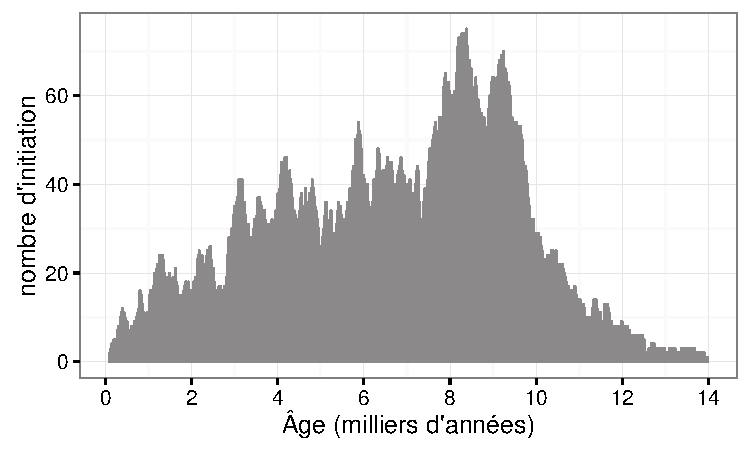
\includegraphics[width=\textwidth]{chap1/holo_peat_ini}
\caption{Nombre de tourbières nouvellement formées pendant l'holocène. Modifié d'après \citep{macdonald2006}.}
\label{fig:holo_peat_ini}
\end{figure}

L'accumulation du carbone nécessite donc que davantage de carbone soit assimilé, par photosynthèse, qu'émis par l'écosystème.
Les tourbières n'assimilent pas le carbone à des vitesses supérieures à d'autres écosystèmes.
En comparaison avec un sol forestier la production primaire est plus faible \plop.
Ce n'est donc pas en assimilant d'avantage de carbone que les tourbières l'accumulent, mais en diminuant les sorties
%Si les entrées de carbone ne sont pas supérieures à d'autres écosystèmes, il faut donc que les sorties soient plus faibles.
C'est en effet parce que les matières organiques produites par ces écosystèmes sont moins dégradées que dans d'autres que le carbone s'accumule.
Ceci est rendu possible par les niveaux de nappe élevés de ces écosystèmes, minimisant les processus de dégradation aérobie en limitant l'accès à l'oxygène.
Cet effet est de plus renforcé par la végétation spécifique de ces écosystèmes, les sphaignes, qui produisent des litières difficilement dégradables, dite récalcitrantes, par rapport à celles produites par les végétaux vasculaires \citep{hobbie1996,liu2000}.
La vitesse de décomposition relative entre les différentes espèces de sphaignes est mal connue \citep{cornelissen2007}.
Des différences ont été observées entre espèces pour les parties jeunes de la plante, mais la différence est moindre pour les parties plus anciennes \citep{limpens2003}.

%C'est cette fonction de puits de carbone qui rend l'importance de ces écosystèmes non négligeable malgré la faible surface qu'ils représentent.
%Les estimations du stock de carbone présent dans les tourbières tempérées/boréales sont comprises entre 270 et \SI{455}{\giga\tonne\,C} \citep{gorham1991,turunen2002}.
%Les différences entre les estimations sont liées aux incertitudes de cartographie citées précédemment auxquelles s'ajoutent des incertitudes concernant l'épaisseur et la densité moyenne de la tourbe.
%Le carbone stocké dans les tourbières représente 10 à \SI{25}{\percent} du carbone présent dans les sols et entre 30 et \SI{60}{\percent} du stock de carbone atmosphérique.

\begin{table}
\centering
\caption{Estimations des stocks de C pour différents environnements}
\label{table:CCycleStocks}
\begin{tabular}{llp{7cm}}\toprule
Compartiment & Stock (en Gt de C) & référence \\ \midrule
Tourbières & 270 -- 455 & \cite{gorham1991,turunen2002} \\ 
Végétation & 450 -- 650 & \cite{Robert2003}\\ 
Sols & 1500 -- 2000 & \cite{Robert2003,Post1982,Eswaran1993}\\ 
\coo atmosphérique & 750 -- 800 & \cite{Robert2003}\\ 
Permafrost & 1700 & \\ 
\bottomrule
\end{tabular}
\end{table}

%Ce stock est un héritage datant des 10 derniers milliers d'années, l'holocène, période pendant laquelle se sont formés la majorité des tourbières \plop \citep{yu2010}.
%Le fonctionnement naturel de ces écosystèmes permet le stockage du C.
%C'est un des services écologiques que rendent les tourbières et que l'on appelle la fonction puits de carbone.
%Cette fonction est liée an niveau élevé de la nappe d'eau, qui rend l'accès à l'oxygène est plus difficile diminuant d'autant l'activité aérobie, dont la respiration des micro-organismes et des plantes.
%Cela ce traduit par une dégradation relativement faible des matières organiques.
%Elle est également liée à la production de litière récalcitrante par les bryophytes.
%
%En comparaison avec un sol forestier, l'accumulation de matières organiques n'est donc pas lié à une production primaire plus forte, mais bien à une dégradation des matières produites plus faible.
%
%Ces perturbations peuvent induire des modifications de fonctionnement, notamment l'envahissement de ces écosystèmes par une végétation vasculaire, et changer cette fonction puits.

%\subsection{Le cycle global}
%
%Au cours des temps les tourbières ont donc accumulé du carbone... stock
%La vitesse de stockage a pu varier au cours du temps mais elle est estimé à XXXX, ainsi la majorité des tourbières actuelles ont un stock qui remonte à quelques milliers d'années.
%Les estimations précise du stock de C présent dans ces écosystèmes sont délicates, à la fois car la définition de ce qu'est une tourbière que varier selon les régions, mais également car leur étendue exacte n'est pas triviale à estimer, pas davantage que leur profondeur moyenne.
%Cependant il est usuellement admis que le stock de carbone se situe entre 270 et 500 Gt de C
%Les tourbières ont donc accumulées du carbone au cours des 10 derniers milliers d'années.
%Pour ce faire il a donc fallu que davantage de carbone soit capturé que de carbone libéré par l'écosystème.

\subsubsection{Biodiversité dans les tourbières}

%\subsection{Les tourbières, des écosystèmes particuliers}

%\subsubsection{Biodiversité}

%Ces écosystèmes sont le siège d'une biodiversité spécifique relativement importante et rendent un certain nombre de services écologiques.
%Parmi la végétation caractéristique de ces écosystèmes, les sphaignes, des bryophytes (des mousses) sont normalement présentes en abondance.
%Les sphaignes ont quelques particularités qu'il convient de mentionner.
%Ce sont des espèces ingénieures, capable de modifier le milieu dans lequel elle vivent afin de l'adapter à leur besoin.
%Plus spécifiquement elles sont capable d'acidifier leur milieu, de capter les nutriments provenant de l'eau de pluie et de les séquestrer afin de défavoriser d'autres végétaux.
Les tourbières sont le siège d'une biodiversité importante et spécifique, avec en premier lieu les sphaignes qui en plus de produire des litières récalcitrantes ont d'autres spécificités : 
ces bryophytes, ces mousses sont des espèces dites ingénieures, capables de modifier l'environnement dans lequel elles vivent afin de l'adapter à leurs besoins.
Les sphaignes sont ainsi capables d'abaisser le pH, de capter des nutriments et de les séquestrer et ce même quand elles n'en ont pas besoin afin d'empêcher d'autres espèces notamment vasculaires d'en profiter.
Plus précisément, le fait que les sphaignes captent les nutriments via leur capitulum leur permet d'intercepter les nutriments avant qu'ils ne soient captés par d'éventuelles racines positionnées plus bas \citep{malmer1994,svensson1995}.
%Les sphaignes, comme de nombreuse mousses ont des litières relativement récalcitrantes\footnote{il est d'usage de parler de litières récalcitrantes sans plus de précision. Il s'agit en fait de litières difficilement dégradables} \citep{hobbie1996,liu2000}.
Ces écosystèmes abritent par ailleurs une grande variété de plantes, de micro-organismes (bactéries et champignons) et d'animaux (insectes, vers, amphibiens, oiseaux...).

\subsubsection{Autres fonctions environnementales}

Les tourbières jouent également un rôle important vis-à-vis de la qualité de l'eau, notamment en filtrant les matières en suspension et en dégradant certains micro-polluants organiques.
Elles permettent également de tamponner les effets d'une sécheresse ou d'une inondation en fournissant un peu d'eau dans le premier cas et en retenant une partie des excédents dans le second \citep{joosten2002,parish2008}.

\subsection{Les tourbières et les changements globaux}
On définit les changements globaux comme l'ensemble des modifications environnementales plus ou moins rapides, ayant lieu à l'échelle mondiale, quelle que soit leur origine. Les deux contraintes développées dans cette partie sont la pression de l'homme : contrainte anthropique, et celle du climat : contrainte climatique.
\index{changements globaux}

\subsubsection{Les contraintes anthropiques}
\index{tourbières!utilisation} 

Les interactions entre les Hommes et les zones humides au sens large et les tourbières en particulier remontent probablement à l'aube de l'humanité.
Des chemins de rondins néolithique aux crannogs de l'époque romaine \citep{buckland1993}, de grandes découvertes archéologiques ont été faites dans les écosystèmes tourbeux témoins d'époques révolues.
L’utilisation de la tourbe et des tourbières a dû commencer relativement tôt, mais c'est à partir du 17\textsuperscript{e} siècle que le drainage de ces écosystèmes, pour les convertir en terres agricoles, s'est intensifié.
Au 19\textsuperscript{e} siècle, l'apparition de machines permettant une récolte industrialisée de la tourbe a développé son utilisation comme combustible.
Enfin depuis le milieu du 20\textsuperscript{e} siècle une part importante de ces écosystèmes a été drainée pour développer la sylviculture.
Aujourd'hui l'exploitation principale de la tourbe est liée à son utilisation comme substrat horticole \citep{lappalainen1996,chapman2003}.
Ces utilisations les ont fortement perturbés car elles nécessitent généralement de drainer ces écosystèmes, notamment pour pouvoir y faire rouler des engins mécanisés.
%Ces utilisations nécessitant souvent le drainage des écosystèmes, notamment pour pouvoir y faire rouler des engins mécanisés, les ont fortement perturbés.
Aujourd'hui la surface de tourbières altérées est estimée à \SI{500000}{\square\kilo\metre} environ, principalement du fait de leur reconversion pour l'agriculture et la sylviculture (Tableau~\ref{table:tourbeUsage}).
En France, suite à leur utilisation, principalement agricole, la surface des tourbières a été divisée par deux entre 1945 et 1998, passant de \SI{1200}{\square\kilo\meter} à \SI{600}{\square\kilo\meter} \citep{lappalainen1996,manneville1999}.

Ces écosystèmes ont donc été et sont encore perturbés par différentes activités humaines.
Leur importance est cependant reconnue et elles sont l'objet de nombreuses actions de préservation et/ou de réhabilitation.
\begin{table}[]
\centering
\caption{Surface de tourbe utilisée selon les usages considérés (tourbières non-tropicales). Modifié d'après \citet{joosten2002}.}
\label{table:tourbeUsage}
\begin{tabular}{lll}\toprule
Utilisation & Surface (\si{\square\kilo\meter})  & proportion (\%) \\ \midrule
Agriculture & \num{250000} & \num{50} \\ 
Sylviculture & \num{150000} & \num{30}\\ 
Extraction de tourbe & \num{50000} & \num{10}\\ 
Urbanisation & \num{20000} & \num{5}\\ 
Submersion & \num{15000} & \num{3}\\ 
Pertes indirectes (érosion, ...) & \num{5000} & \num{1}\\[1ex]
Total & \num{490000} & \num{100}\\
\bottomrule
\end{tabular}
\end{table}


\subsubsection{Les contraintes climatiques}

Comme indiqué précédemment, le stock de carbone des tourbières s'est majoritairement constitué pendant l'Holocène.
À cette époque déjà ces écosystèmes étaient influencés par le climat, et leur développement n'a pas été linéaire sur les douze derniers milliers d'années.
Il est reconnu que le développement des tourbières est très important au début de cette période \citep{smith2004,macdonald2006,yu2009}.
Plus particulièrement, entre \num{12000} et \num{8000} ans on recense la plus grande proportion d'initiation de tourbières (Figure~\ref{fig:holo_peat_ini}).
Cette période coïncide avec le maximum thermique holocène (HTM), période pendant laquelle le climat était plus chaud qu'aujourd’hui \citep{kaufman2004}.
Ce constat peut sembler paradoxal : en effet, dans la littérature concernant les tourbières et le réchauffement climatique actuel, il est craint que ces écosystèmes ne deviennent des sources de carbone.
% si l'on considère que dans la littérature concernant les tourbières et le réchauffement actuel, la crainte de voir ces écosystèmes se transformer en source de C est majoritaire.
Cependant ces même auteurs qui ont montré cette relation entre le HTM et le développement important des tourbières, ne préjugent pas de l'effet du réchauffement actuel.
Notamment \citet{jones2010} expliquent que pendant cette période de maximum thermique, il existe également une saisonnalité très importante, avec des été chauds et des hivers froid, qui a dû en minimisant la respiration hivernale de ces écosystèmes, jouer un rôle important dans leur développement.
Cette forte saisonnalité n'est pas attendue lors du réchauffement actuel.
L'effet estimé sous les hautes latitudes semble plus important pendant l'hiver et l'automne, et tendrait donc à minimiser cette saisonnalité \citep{christensen2007}.
Les effets directs attendus du réchauffement sous les hautes latitudes à l'horizon 2100, sont une augmentation des températures de 2 à \SI{8}{\degreeCelsius} dans les zones boréales, et de 2 à \SI{6}{\degreeCelsius} dans les zones tempérées, ainsi  qu'une augmentation probable des précipitations (Figure~\ref{fig:ipcc2013_T_rain}).
De façon plus indirecte est attendue la fonte du permafrost, l'augmentation de l'intensité et de la fréquence de feux et des changements dans les compositions des communautés végétales \citep{christensen2013,frolking2011}.

%L'impact anthropique direct n'est par la seule perturbation auxquelles sont soumises les tourbières.
%D'après les modèles de prédictions du GIEC, les tourbières, comme de nombreux autres écosystèmes, vont subir un changement climatique important dans les années à venir.
%Toujours d'après le GIEC, les changements les plus rapides que ce soit en terme de précipitations ou de température sont à attendre dans les zones boréales là ou se situent la majorité des tourbières.
%De ce constat découle un certain nombre de questions concernant ces écosystèmes.
%D'abord quel effet auront les changements climatiques et avec quelle variabilité régionale ?
%Cette question n'est pas évidente (paradoxe du sol plus froid ? augmentation photosynthèse)
%Quelle sera la sensibilité des tourbières ?
%Là encore leur diversité, leur répartition géographique rend difficile la réponse à cette question.
%Enfin découlant des précédentes, qu'elle est le devenir de la fonction puits de carbone.



\begin{figure}
\centering
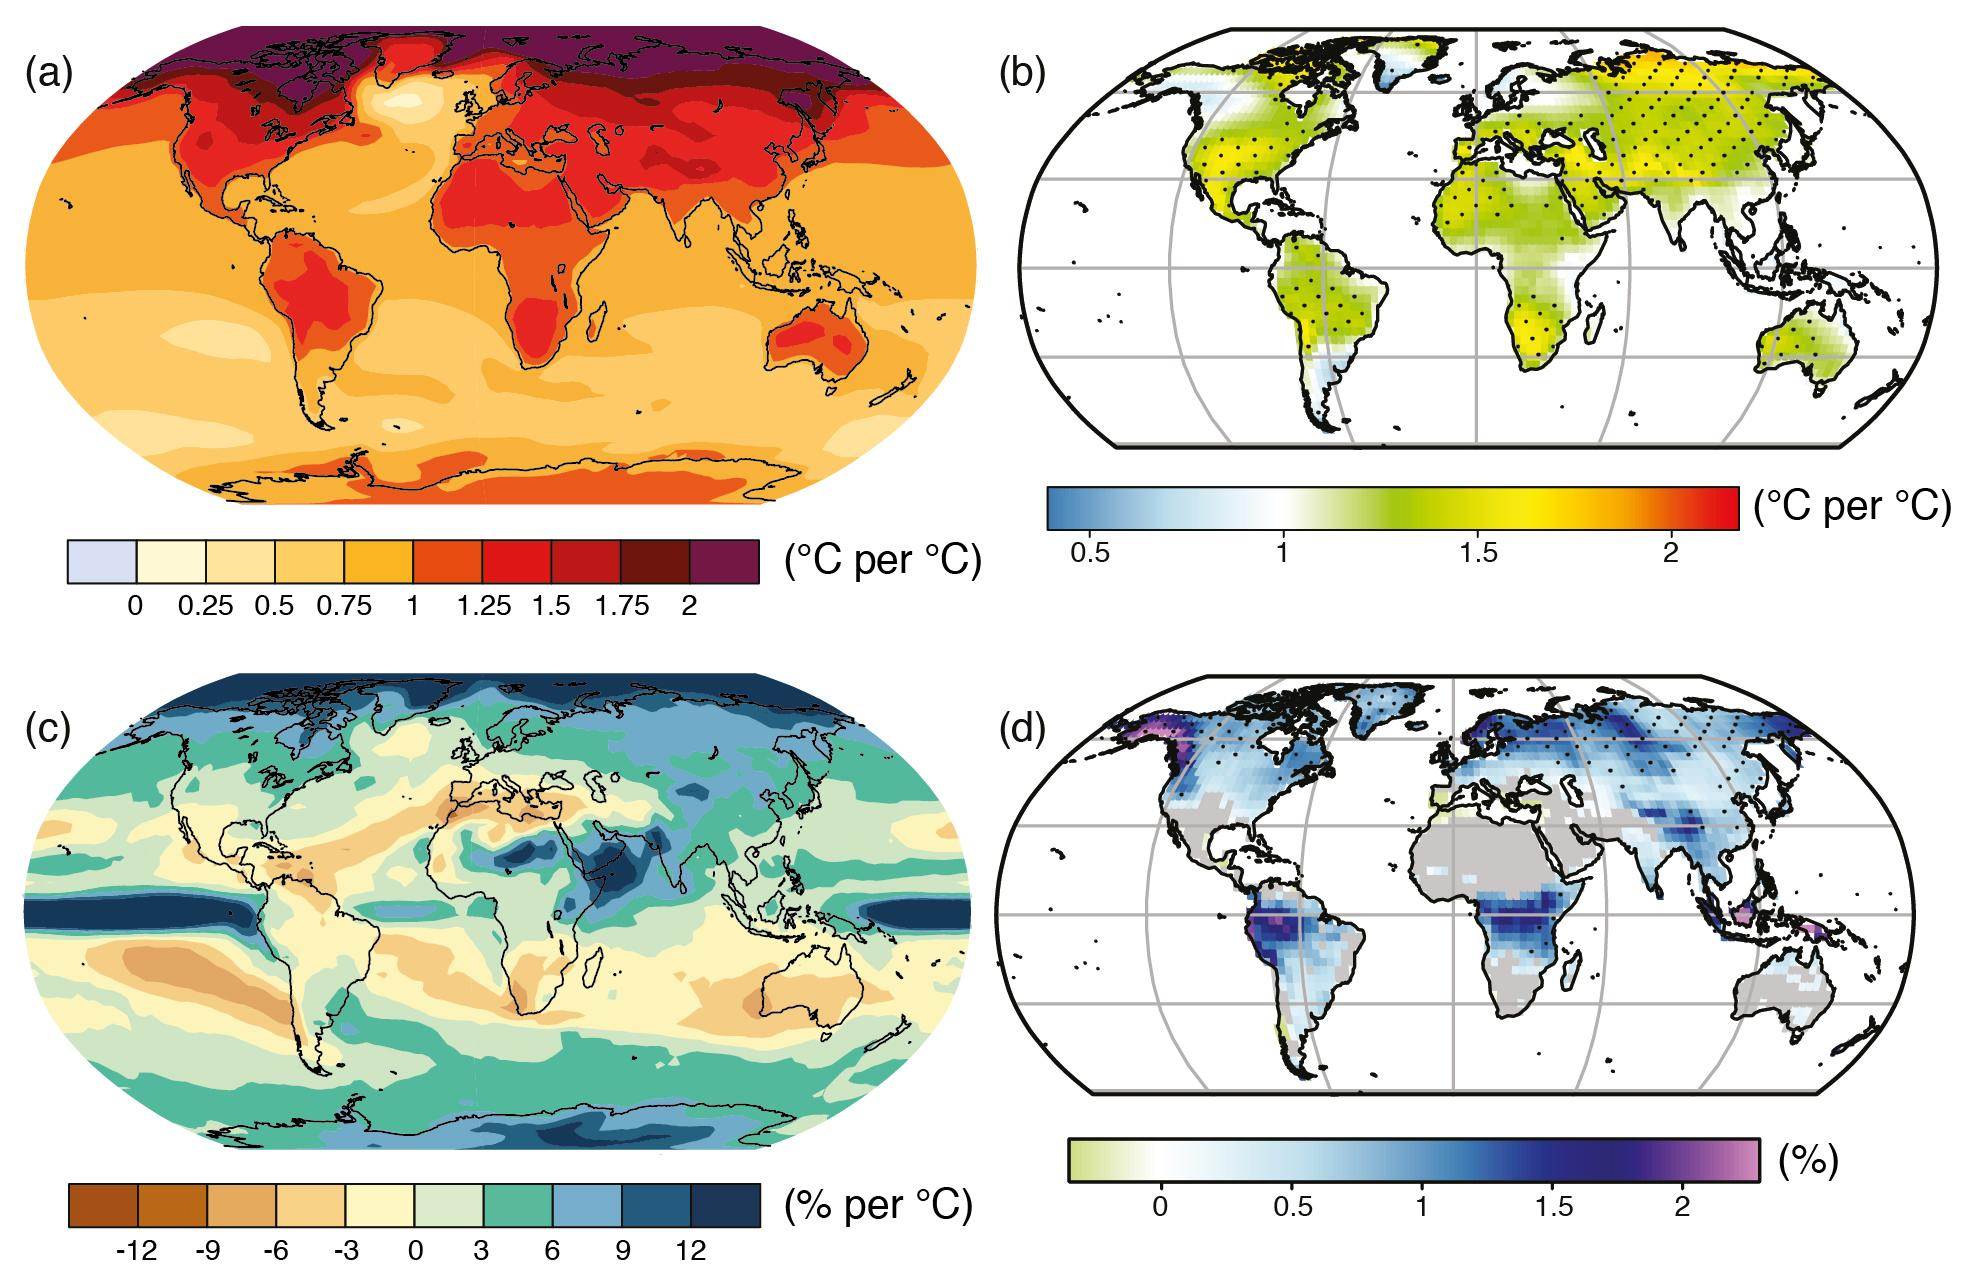
\includegraphics[width=\textwidth]{chap1/ipcc2013_RCP45}
\caption{Projection des changements à l'horizon 2100, des moyennes et extrêmes annuels (sur terre) des températures de l'air et des précipitations : (a) température de surface moyenne par \si{\degreeCelsius} de changement global moyen, (b) 90\textsuperscript{e} percentile des températures journalières maximum par \si{\degreeCelsius} de changement de température moyenne maximale, (c) précipitations moyenne (en \si{\percent} par \si{\degreeCelsius} de changement de température moyenne) et (d) fraction de jours ayant des précipitations dépassant le 95\textsuperscript{e} percentile. Sources : (a) et (c) simulations CMIP5, scénario RCP4.5, (b) et (d) adaptation d'après \citet{orlowsky2012}(\textbf{IPCC2013}).}
\label{fig:ipcc2013_T_rain}
\end{figure}

%Toutes ces perturbations posent notamment la question de la pérennité de la fonction puit de carbone de ces écosystèmes.

Les tourbières, qui ont accumulé un stock de carbone important, sont donc soumises à des contraintes fortes qu'elles soient anthropiques ou climatiques.
Afin de mieux comprendre le devenir de ce carbone, l'étude de ces écosystèmes, des flux de carbone qu'ils échangent avec l'atmosphère, est une nécessité.

\index{tourbières|)}

\section{Flux de gaz à effet de serre et facteurs contrôlants}

Cette partie s'attache à décrire les gaz à effet de serre (GES) et leurs liens avec les tourbières, les flux de carbone et les processus qui y sont liés, puis les facteurs contrôlant les flux de l'échelle des processus jusqu'aux individus et communautés (nécessaire afin de pouvoir appréhender correctement les flux à des échelles plus large), les facteurs contrôlant à l'échelle de l'écosystème (colonne de tourbe, site complet) et enfin les bilans de carbone.


\subsection{GES et tourbières}

Dans l'atmosphère le carbone est principalement présent sous forme de dioxide de carbone (\coo) et de méthane (\chh).
La concentration en \coo dans l'atmosphère fluctuait avant l'ère industrielle entre 180 et \SI{290}{ppm}.
En 1750 au début de l'ère industrielle sa concentration était de \SI{280}{ppm} environ avant d'augmenter pour atteindre \SI{391}{ppm} aujourd'hui (moyenne annuelle en 2011) \citep{Ciais2014}.
Différents processus naturels permettent d'extraire du \coo de l'atmosphère : la photosynthèse, la dissolution du \coo dans l'océan et enfin l'altération de silicate et les réactions avec le carbonate de calcium.
Ces processus s'effectuent à des échelles de temps différentes, en conséquence après une émission de \coo, il ne reste que \SI{40}{\percent} après \SI{100}{ans}, mais plus de \SI{20}{\percent} après \SI{1000}{ans} et plus de \SI{10}{\percent} après \SI{10000}{ans} \citep{joos2013,Ciais2014} (Figure~\ref{fig:co2_decroissance}).

\begin{figure}
\centering
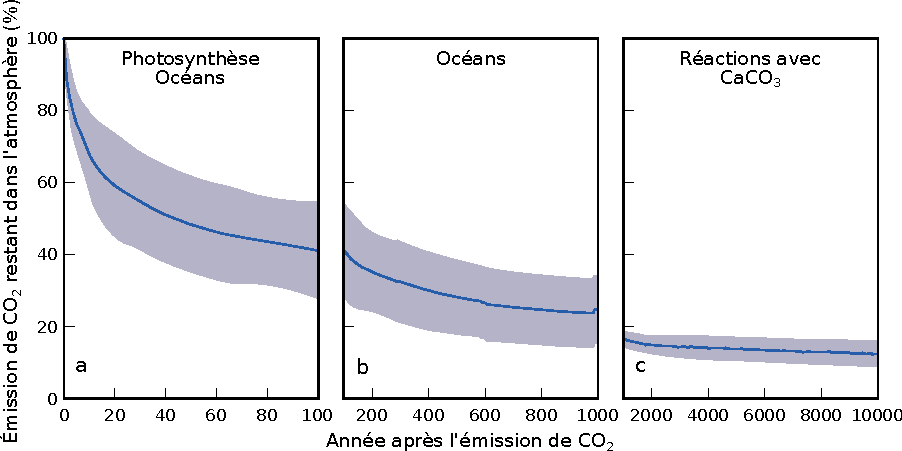
\includegraphics[width=\textwidth]{chap1/co2_decroissance}
\caption{Décroissance de la proportion de \coo de l'atmosphère suite à une émission idéalisée de \SI{100}{\peta\gram C}. les graphes (a) et (b) sont une moyenne de modèles \citep{joos2013}, le graphe (c) est une moyenne d'autres modèles \citep{archer2009}. Modifié d'après \citep{Ciais2014}.}
\label{fig:co2_decroissance}
\end{figure}


La concentration en \chh dans l'atmosphère est estimée à \SI{350}{ppb}\footnote{Partie par milliard (\textit{part per billion} en anglais)} il y a \SI{18000}{ans} environ lors de la dernière glaciation et à \SI{720}{ppb} en 1750.
En 2011 elle est estimée à \SI{1800}{ppb} \citep{Ciais2014}.
À l'inverse du \coo sa durée de vie dans l'atmosphère est limitée : moins de \SI{10}{ans} \citep{lelieveld1998,prather2012}.
Cependant son potentiel de réchauffement global\footnote{indice permettant de comparer le pouvoir de réchauffement des différents GES en donnant une équivalence par rapport au \coo. Le PRG du \coo vaut donc 1 par définition.} (PRG) est important notamment à court terme, 72 à 20 ans.
À plus long terme son effet relativement au \coo diminue et atteint 25 à l'horizon 100 ans.
Les zones humides sont la première source naturelle de \chh atmosphérique avec un flux à l'échelle globale estimé entre \num{145} et \SI{285}{\tera\gram\per\year} \citep{lelieveld1998,wuebbles2002,Ciais2014} \textbf{(Tableau ?)}.
Les tourbières de l'hémisphère nord comptent pour \SI{46}{\tera\gram\per\year} \citep{gorham1991} \textbf{(pas de source plus récente ?)}.


À l'échelle globale, le stockage de C par les tourbières, prenant en compte à la fois le \coo et le \chh, est estimé à \SI{70}{\tera\gram\per\year} \citep{clymo1998}.

\subsection{Les flux de GES entre l'atmosphère et les tourbières}

\subsubsection{De l'atmosphère à l'écosystème}

\begin{figure}
\centering
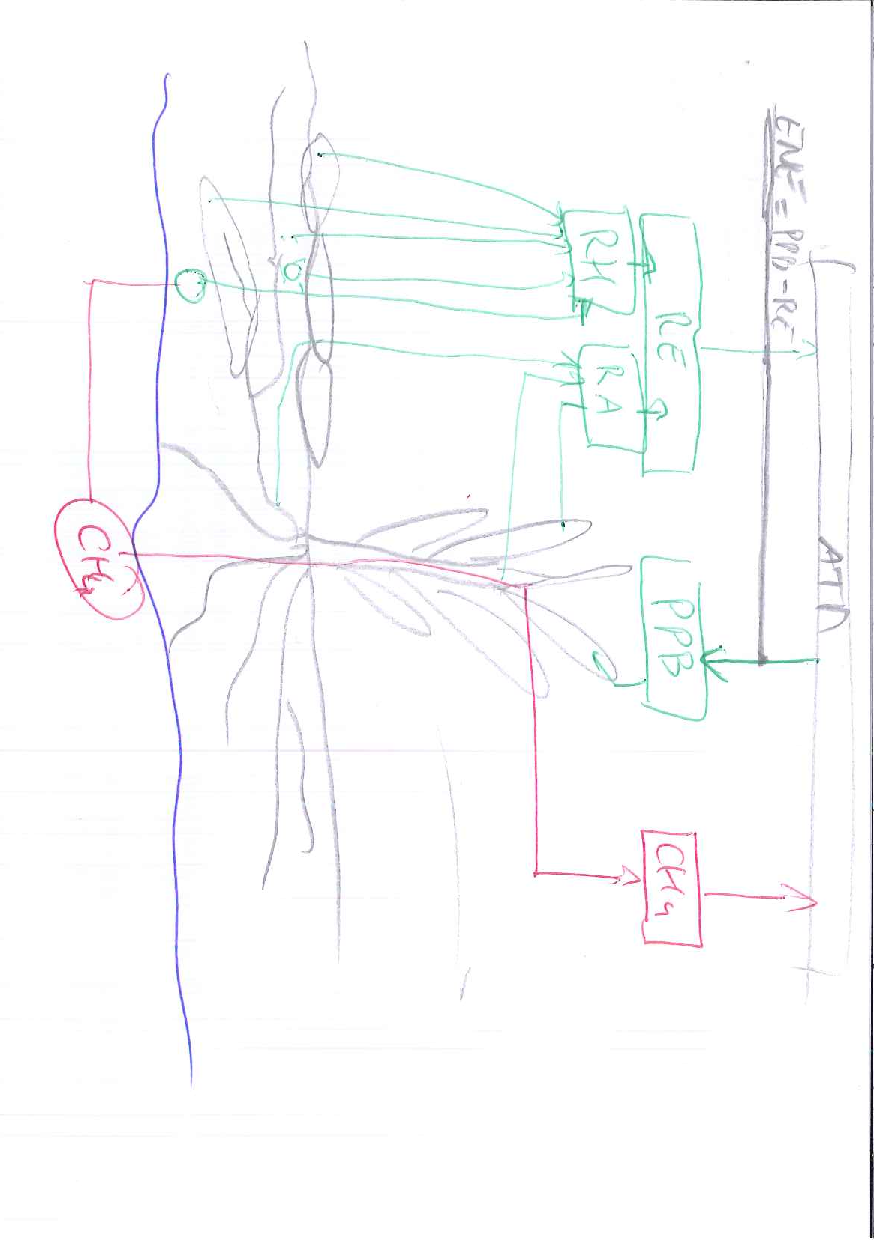
\includegraphics[width=\textwidth]{chap1/ges_flux}
\caption{schéma des flux de carbone entre une tourbière et l'atmosphère}
\label{fig:ges_flux}
\end{figure}

Avant de stocker et de conserver du carbone, le faut le capturer.
Ce transfert du carbone de l'atmosphère à la tourbe se fait par le processus de photosynthèse, où le \coo est assimilé dans la matière organique.
Principalement par les végétaux vasculaires et les mousses, et éventuellement, bien que dans de moindre proportions, par des algues, des lichens ou des bactéries photosynthétiques \citep{girard2011}.
On peut écrire la réaction de photosynthèse de la façon suivante : 

$$\begin{aligned}
CO_{2} + H_{2}O + photons &\rightarrow CH_{2}O + O_{2}\\
\end{aligned} $$

Si la photosynthèse est le processus majeur d'assimilation du \coo, il existe d'autres voies métaboliques permettant la capture du \coo de l'atmosphère.\index{photosynthèse}
Par exemple les micro-organismes chemolithotrophes (\textbf{expliciter}) sont capables d'assimiler le \coo en utilisant l'énergie issue de l'oxydation de composés inorganiques, ce que l'on appelle la chimiosynthèse, mais leur importance est moindre.

On définit la \textbf{Production Primaire Brute} (PPB), \textit{Gross Primary Production}, (\textit{GPP}) comme :

\begin{pdef}
\textsc{Production Primaire Brute (PPB)} :

Quantité de carbone extraite de l'atmosphère et transformée en matières organiques par l'écosystème principalement via la photosynthèse.
Ce flux est exprimé en quantité de carbone par unité de surface et de temps.
\end{pdef}

Les tourbières sont des écosystèmes dont la production primaire est estimée à environ \SI{500}{\gcm} ;
la production de la strate muscinale pouvant atteindre \SI{80}{\percent} \citep{francez2000}.
Les productions primaires dans les tourbière ne sont pas élevées \plop.
C'est la faible décomposition des matières organiques qui permet aux tourbières de stocker du carbone.
%L'accumulation moyenne estimée dans les tourbières boréales est de \SI{30}{\gcm}. Le taux d'accumulation varie en fonction des espèces végétales présentes (\plop), le niveau d'eau (\plop), ... (??)
Du fait de la production élevée de \chh dans les tourbières, il n'y a pas de flux direct de \chh de l'atmosphère vers cet écosystème.
\SI{90}{\percent} du \chh présent dans l'atmosphère est extrait via des réactions avec des radicaux hydroxyles ayant lieu majoritairement dans la troposphère.

\subsubsection{De l'écosystème à l'atmosphère}

Les sources de carbone émises par les tourbières vers l'atmosphère sont multiples.
D'abord différents gaz peuvent être émis, notamment le \coo et le \chh des molécules de carbone organique volatiles.
Le processus majeur de production de \coo se fait par respiration qui, au niveau cellulaire, peut être écrit sous la forme :

$$\begin{aligned}\label{eq:respi}
C_{6}H_{12}O_{6} + 6O_{2} &\rightarrow 6CO_{2} + 6H_{2}O \\
\end{aligned} $$

Ce gaz est produit principalement par la respiration aérobie et minoritairement par les respirations anaérobies, par fermentations (e.g. du glucose, de l'acétate), ou encore par oxydation du \chh \citep{lai2009}.
Les principales sources d'émissions du \coo sont représentées dans la figure~\ref{fig:ges_flux}.
À l'échelle macroscopique la respiration est séparée en deux.
D'un côté la respiration végétale (des feuilles, des tiges, des racines) que l'on appelle la \textbf{respiration autotrophe\footnote{Production de matières organiques à l'aide de composés minéraux simples.}}.
De l'autre, rassemblé sous le terme de \textbf{respiration hétérotrophe}\footnote{Production de matières organiques à partir de substrats organiques.}, la respiration du sol, liée à l'excrétion d'exsudats par les racines, la décomposition des litières et des matières organiques par les micro-organismes et l'oxydation du \chh par les organismes méthanotrophes.
%e la rhizosphère, liée à l'émission d'exsudats par les racines, la décomposition des litières et des matières organiques, la respiration de la faune et l'oxydation du \chh par les organismes méthanotrophes.
L'ensemble de ces respirations est défini comme : 
\begin{pdef}
\textsc{Respiration de l'Écosystème (RE)} :

%\hfill{\textit{Gross Primary Production (GPP)}}\\
Quantité de carbone émise sous forme de \coo par l'écosystème dans l'atmosphère. 
Elle englobe la respiration autotrophe et hétérotrophe en incluant ses composantes aériennes et souterraines.
Ce flux est exprimé en quantité de carbone par unité de surface et de temps.
\end{pdef}
\index{respiration!de l'écosystème}
On distingue la respiration de l'écosystème de celle du sol en définissant la respiration du sol (RS) comme l'ensemble des respirations de la colonne de sol, à l'exclusion de la partie aérienne \citep{luo20063}.\index{respiration!du sol}
Cependant, dans la littérature la respiration du sol peut parfois être assimilée à la respiration de l'écosystème (RE)\citep{raich1992}.
Les études discriminant RS et RE montrent ainsi que dans des sols tourbeux, RS compte pour plus de \SI{60}{\percent} de RE \cite{lohila2003}.
%
%Une autre source de \coo est l'oxydation du \chh lors de sa migration des zones anoxiques aux zones oxiques de la colonne de tourbe.
%Enfin dans les zones anaérobie, le \coo peut être produit par fermentation (respiration anaérobie).
La production de \coo est donc un signal multi-sources intégré sur l'ensemble de la colonne de tourbe.
Le transport du \coo produit se fait par diffusion suivant le gradient de concentration, fort dans le sol et plus faible dans l'atmosphère.
C'est cette multitude de processus qui rend l'estimation de ce flux difficile.
En effet chacune des respirations n'aura pas la même sensibilité vis à vis de facteurs contrôlant.
%La respiration de l'écosystème (RE) est définie comme l'ensemble des respirations de la colonne de tourbe, en incluant à la fois sa partie aérienne et sa partie souterraine. \index{respiration!de l'écosystème}
%La respiration du sol (SR) est elle définie comme l'ensemble des respirations de la colonne de tourbe, en excluant la partie aérienne.\index{respiration!du sol}
%La respiration du sol comprend donc principalement les respirations issues de la rhizosphère et des communautés de micro-organisme.

%Les tourbières sont des écosystèmes dont la production primaire est estimée à environ \SI{500}{\gcm} \cite{francez2000}. 



Conséquence du niveau de nappe élevé des tourbières, le développement d'une zone anoxique importante dans la colonne de sol favorise la production de \chh.
Il est produit par des \textit{Archaea} méthanogènes, des organismes anaérobies vivants sous le niveau de la nappe.
En moyenne les flux de \chh mesurés dans les tourbières s'étendent de 0 à plus de \SI{0.96}{\uml}, avec généralement des flux compris entre \num{0.0048} et \SI{0.077}{\uml} \citep{blodau2002}.
Le \chh est principalement produit à partir d'acétate (CH\textsubscript{3}COOH) ou de dihydrogène (H\textsubscript{2}) + \coo, ces deux composés étant dérivés de la décomposition préalable de matières organiques \citep{lai2009}.

$$\begin{aligned}
CH_{3}COOH  &\rightarrow CH_{4} + CO_{2}\\
4H_{2} + CO_{2} &\rightarrow CH_{4} + 2H_{2}O\\
\end{aligned} $$
Le \chh produit est transporté dans l'atmosphère par diffusion, ébullition ou à travers certaines plantes \citep{joabsson1999,colmer2003}.
Pendant son transport, le \chh peut être oxydé par des organismes méthanotrophes.
Cette transformation produit tour à tour différents composés (méthanol, formaldéhyde, formate) aboutissant à la production de \coo \citep{whalen2005}.

$$
CH_{4} \rightarrow CH_{3}OH \rightarrow HCHO \rightarrow HCOOH \rightarrow CO_{2} \\
$$

On définit le flux de \chh comme : 
\begin{pdef}
\textsc{Flux de \chh (\fchh)} :

%\hfill{\textit{Gross Primary Production (GPP)}}\\
Quantité de carbone émise sous forme de \chh par l'écosystème dans l'atmosphère, suite au bilan des processus de création et de destruction de la molécule.
Ce flux est exprimé en quantité de carbone par unité de surface et de temps.
\end{pdef}

%Sa variabilité est donc fonction des conditions environnementales, des communautés (principalement microbiennes et végétales) impliqués 



Au final, on peut noter que si le flux de carbone de l'atmosphère à l'écosystème a pour source quasiment unique la réaction de photosynthèse des plantes, le flux de carbone de l'écosystème vers l'atmosphère est multi-source avec un nombre important de réactions de respirations et de fermentations.
La variabilité du premier flux résulte majoritairement de la nature et la structure des communautés végétales et de leurs sensibilités aux conditions environnementales.
Celle du second flux est multiple et est liée à la diversité des réactions permettant la dégradations des matières organiques et des communautés végétales ou microbiennes impliquées, de leur sensibilité aux conditions environnementales.

\subsection{Les facteurs majeurs contrôlant les flux de GES}

Dans cette partie seront décrits les facteurs qui contrôlent les flux de carbone en commençant à une échelle relativement fine pour atteindre celle de l'écosystème qui nous intéresse plus particulièrement.
%Cette échelle inclut la colonne de tourbe, le mésocosme, en tant que partie d'un ensemble plus vaste, en tant que sous-écosystème. 
%Elle inclut forcément l'écosystème dans son sens général, regroupant les écosystèmes tourbeux mais également l'écosystème au sens plus spécifique de l'entité étudiée.

Les facteurs majeurs qui contrôlent les flux de carbone sont globalement connus.
Comme bon nombre de réactions biochimiques, les vitesses de réactions des processus décrits précédemment sont fonction de la \textbf{température}.
Cette relation  a été mise en évidence par un chimiste suédois en 1889, Svante August Arrhenius, sur la base de travaux réalisés par un autre chimiste, néerlandais, Jacobus Henricus Van't Hoff.
Le \textbf{niveau de la nappe d'eau}, interface entre un monde oxique et un monde anoxique, et la \textbf{teneur en eau du sol} vont également influencer sur ces flux.
Ainsi que la végétation  que ce soit de façon directe comme siège de la photosynthèse et de la respiration autotrophe, ou indirecte en fournissant des nutriments de son vivant à travers les exsudats racinaires, ou à sa mort en devenant litière.


\subsubsection{Facteurs contrôlant la photosynthèse}
\index{production primaire brute!contrôle}

\begin{figure}
\centering
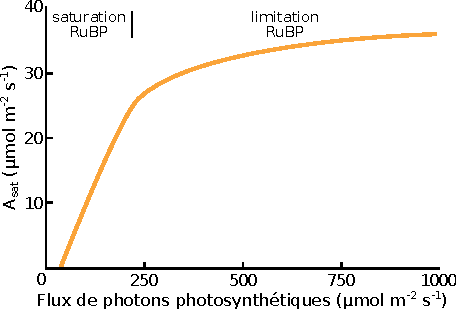
\includegraphics[width=.8\textwidth]{chap1/PAR_photo}
\caption{todo, modifié d'après \citet{long1993}}
\label{fig:PAR_photo}
\end{figure}

À l'échelle des espèces végétales, la quantité de carbone assimilable par la photosynthèse est fonction de la quantité de lumière reçue \citep{long1993}.
La quantité de carbone assimilé augmente d'abord de façon linéaire avec le rayonnement, avant d'être limitée par la régénération d'une enzyme, la Rubisco\footnote{ribulose-1,5-bisphosphate carboxylase/oxygénase}, nécessaire à la fixation du \coo (Figure~\ref{fig:PAR_photo}).
Les limitations de l'assimilation, que ce soit la pente initiale de la partie linéaire, ou l'assimilation maximale, varient de façon importante en fonction de l'espèce végétale considérée \citep{wullschleger1993}.
La régénération de la Rubisco, qui limite la photosynthèse, est contrainte par la capacité de transport des électrons.
La vitesse de ce transport est fonction de la température et est traditionnellement décrite par une équation d'arrhenius modifiée, relativement complexe, ou par une équation simplifiée \citep{farquhar1980,june2004}.
À cette échelle, le niveau de l'eau va également influencer le développement de la végétation en facilitant plus ou moins leur accès à l'eau.
\citet{wagner1984} montrent par exemple que deux espèces de sphaignes ont des tolérances différentes à la dessiccation : l'espèce vivant dans les gouilles est plus résistante que celle vivant sur les buttes.
Dans des conditions expérimentales différentes, lors de re-végétalisation de deux tourbières, \cite{robroek2009} montrent que différentes espèces de sphaignes se développent de façon optimale à différents niveaux de nappe selon leurs affinités.
Cette variabilité entre espèces d'une même famille est elle même mise en évidence par leur variabilité en terme de productivité primaire (Figure~\ref{fig:prod_sphagnum}).
La productivité primaire varie également entre différentes communautés végétales : les bryophytes n'ont pas la même productivité primaire que les graminées ou que les arbustes \citetext{\citealp{moore2002} dans \citealp{rydin2013b}}.
%En plus de ces différences entre groupes de végétaux, il existe également des différences de productivité pour un même groupe selon le type de tourbière \citetext{\citealp{moore2002} dans \citealp{rydin2013b}}.
%\citet{weltzin2000} montrent par exemple que dans les tourbières de haut-marais, les sphaignes et les arbustes ont une productivité importante, les herbacées et graminées ont une productivité beaucoup plus faible.
%À l'inverse ce sont les herbes et les graminées qui ont la plus forte productivité dans les tourbières de bas-marais pauvres.
%devant les sphaignes puis les arbustes.

Le niveau de la nappe d'eau et les propriétés physiques du sol contraignent également la teneur en eau du sol et la hauteur de la frange capillaire.
Cette dernière atteint généralement la surface du sol tant que le niveau de la nappe d'eau ne descend pas en dessous de \num{30} à \SI{40}{\centi\metre} de profondeur \citep{laiho2006}.
La hauteur du niveau d'eau va influencer sur le développement des différentes communautés végétales.
Un niveau d'eau élevé peut diminuer l'accès de la végétation vasculaire à l'oxygène par leur racines alors qu'il sera propice au développement de sphaignes.
À l'inverse un niveau d'eau bas peut faciliter le développement de certains végétaux vasculaires au détriment des bryophytes \plop.
Cette compétition entre espèces végétales peut déterminer l'évolution à long terme des communautés et impacter la PPB.
\citet{gornall2011} montrent que les effets des mousses sur les plantes vasculaires sont en partie positifs et en partie négatifs et que leur «effet net» peu varier, notamment en fonction de l'épaisseur de la strate muscinale.
La composition des communautés végétales va donc avoir un effet sur le potentiel photosynthétique de l'écosystème.
Ce potentiel peut varier selon le végétal considéré et les conditions environnementales dans lesquelles il se trouve \citep{moore2002}.

\begin{figure}
\centering
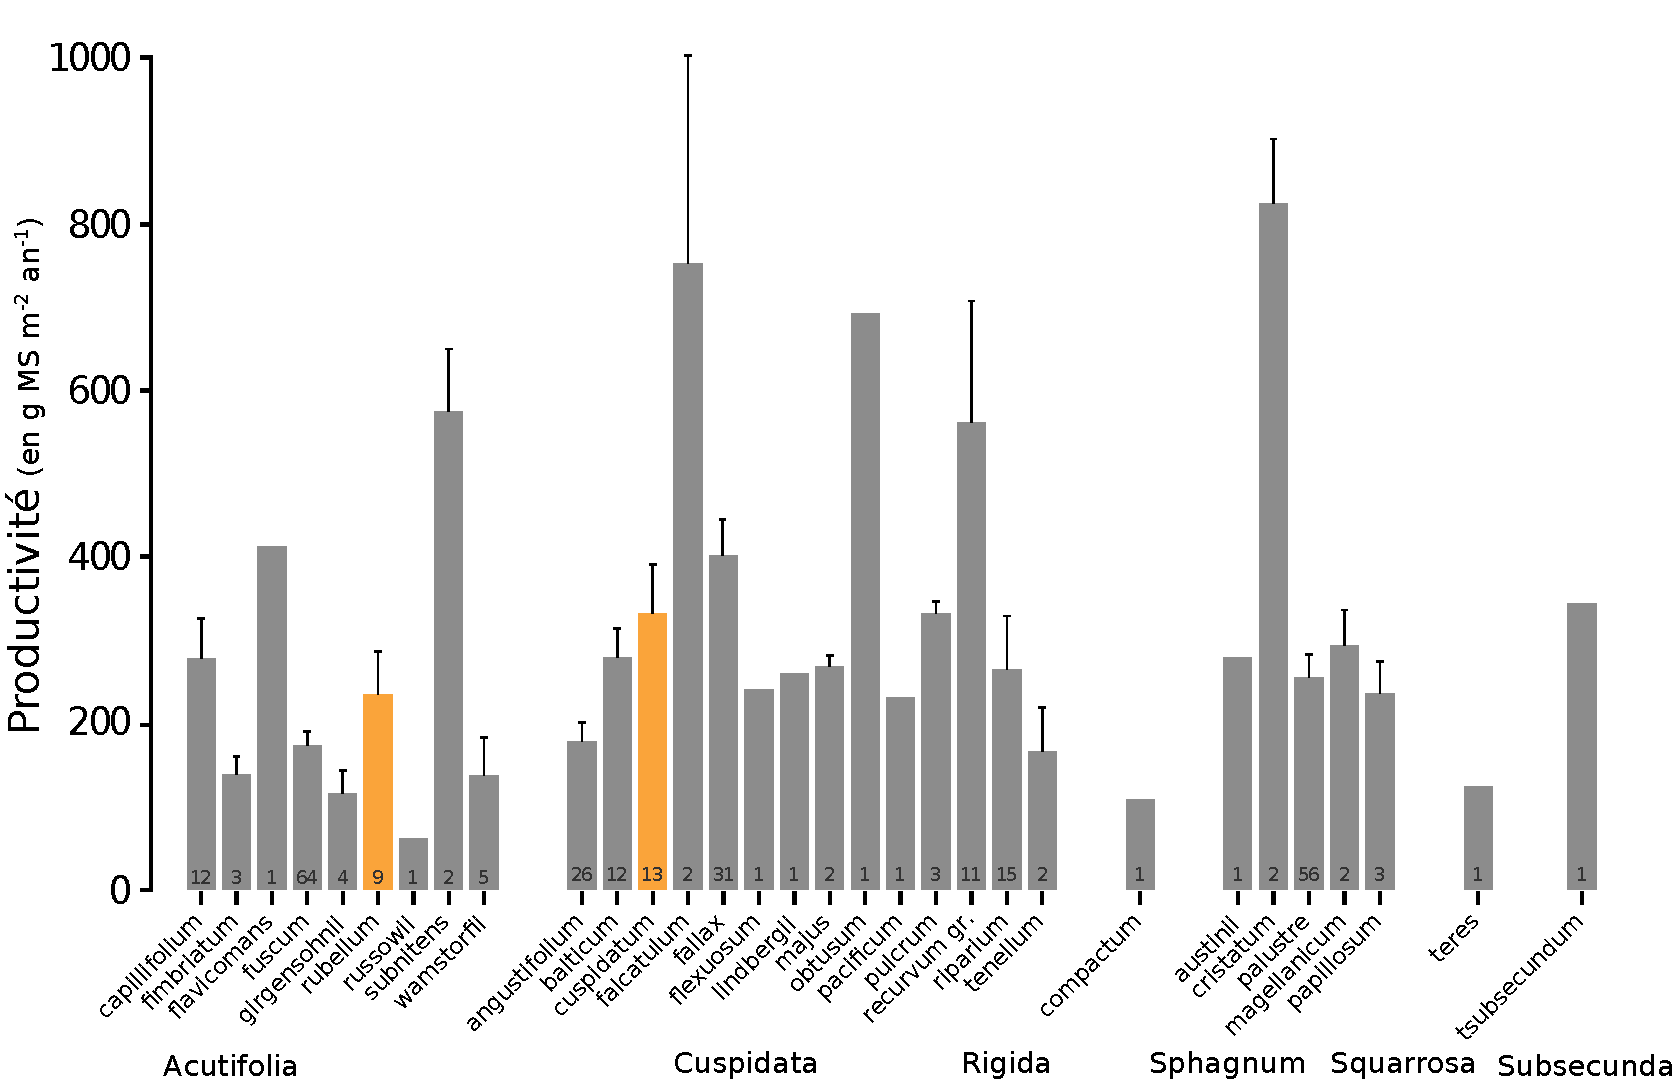
\includegraphics[width=\textwidth]{chap1/prod_sphagnum}
\caption{Productivités moyennes des espèces de sphaignes en \si{\gram\per\square\metre\per\year}. Les barres d'erreurs représentent l'erreur standard. Le nombre d'observation est indiqué par les nombres à l'intérieur des barres. Les espèces en orange sont celles rencontrées sur le site d'étude. Modifié d'après \citet{gunnarsson2005}}
\label{fig:prod_sphagnum}
\end{figure}

À l'échelle de l'écosystème dans son ensemble la température, la végétation et le niveau de l'eau, co-varient ce qui rend la discrimination de leurs effets respectifs difficile.
L'effet d'une variation de température peut, selon l'échelle de temps considérée, influencer le niveau de nappe et la végétation.
Distinguer ces facteurs n'est pas anodin.
Dans l'optique de discriminer l'effet de chacun de ces facteurs, \citet{munir2015} isolent l'effet de la température en utilisant des OTC\footnote{OTC ou chambres à toit ouvert, ce sont des hexagones en polycarbonate permettant un rehaussement \textit{in-situ} de la température moyenne de l'air.} (\textit{Open Top Chamber}).
%Ces dispositifs ressemblent à des serres ouvertes et permettent de réchauffer une zone de la tourbière.
Ils montrent que le réchauffement par les OTC augmente la PPB.
Néanmoins la majorité des études réalisées sur le terrain montrent les effets de variation de la température et du niveau de la nappe simultanément.
\citet{cai2010} ont par exemple montré que des conditions plus chaudes et sèches d'une année augmentaient la PPB.
Cependant l'effet du niveau de la nappe d'eau peut varier selon le contexte : dans une étude sur les effets à long terme d'une variation du niveau de la nappe, \citet{ballantyne2014} montrent qu'une baisse du niveau de la nappe entraîne une augmentation de la PPB en facilitant l'accès des plantes vasculaires à l'oxygène et aux nutriments.
Paradoxalement, un rehaussement du niveau de la nappe d'eau suite à un stress hydrique prolongé conduit également à une augmentation de la PPB \citep{strack2013}.
Pour un gradient croissant de niveaux de nappe d'eau dans un haut-marais, \citet{weltzin2000} montrent une diminution de la productivité des arbustes, tandis que celle des graminées n'est pas affectée.
À l'inverse, pour un gradient similaire dans un bas-marais, la productivité des arbustes n'est pas affectée tandis que celle des graminées augmente.
Une opposition similaire est également relevée concernant les graminées soumises à un traitement infra-rouge afin de les réchauffer.
La productivité des graminées diminue dans la tourbière de haut-marais et augmente dans la tourbière de bas-marais.
Les effets du niveau de la nappe peuvent donc être variables selon les communautés végétales et le contexte (l'écosystème, le niveau initial) dans lequel elles se trouvent.

\subsubsection{Facteurs contrôlant la RE}
\index{respiration!de l'écosystème!contrôle}

%La respiration, au sens de la réaction biochimique telle que  décrite par l'équation~\ref{eq:respi} est stimulée par la température.
La respiration est limitée par la quantité de substrat (organique labile) et l'accès à l'oxygène.
Dans les tourbières la limitation en substrat n'a de sens que vis-à-vis de communautés spécifiques.
Les substrats facilement utilisables, par exemple les sucres, peuvent devenir limitant \plop.
De part la quantité de matières organiques qu'elles contiennent, les tourbières constituent un vaste réservoir de substrat organique de plus en plus difficile à dégrader avec la profondeur.
Plus les substrats sont facilement utilisables plus leur utilisation est rapide est plus ils risquent de devenir limitant.
Inversement moins les substrats sont dégradables plus leur utilisation est lente et plus ils s'accumulent.
Mais l'accès à l'oxygène rendu difficile par les hauteurs élevées du niveau de la nappe est prépondérant \plop.
La qualité du substrat (la facilité qu'il aura à être dégradé) va donc déterminer la vitesse de respiration.
Par ailleurs la photosynthèse en libérant des substrat, les exsudats racinaires, affecte également la respiration du sol.

%\textbf{Partionnement de la RE}
À l'échelle de l'écosystème de nombreuses études ont mis en évidence une corrélation positive entre la respiration et la température \citep{singh1977,raich1992,luo2006}.
Cependant la diversité cumulée des processus, communautés et des conditions environnementales qui influencent la respiration, font qu'aucune équation ne fait réellement consensus.
Cependant la majorité de ces études décrivent une augmentation exponentielle de la respiration avec la température.
Ainsi dans les tourbières, des observations \textit{in-situ} ont montré que dans des conditions plus chaudes, mais également plus sèches (ces deux conditions sont difficilement séparables sur le terrain) la RE a tendance à augmenter  \citep{aurela2007,cai2010,ward2013}.
D'autres observations sur des mésocosmes\footnote{définition méso} de tourbe ont également montré une relation positive entre les variations de RE et celle de la température \citep{updegraff2001,weedon2013}.

Le niveau de la nappe d'eau conditionne l'accès des micro-organismes à l'oxygène, de ce fait joue un rôle important ; un niveau d'eau qui diminue se traduisant généralement par une hausse de la RE que ce soit à long terme \citep{strack2006,ballantyne2014} ou à plus court terme \citep{aerts1997}.

De façon plus indirecte, le type de végétation influence la vitesse de décomposition des litières \citep{hobbie1996,liu2000,gogo2015}.
La végétation peut également stimuler la respiration des micro-organismes présents dans la rhizosphère\footnote{zone du sol impactée par les racines} via la libération d'exsudats racinaires \citep{moore2002}.

\subsubsection{Facteurs contrôlant l'ENE}
\index{echange net de l'ecosystem@échange net de l'écosystème!contrôle}

À l'échelle de l'écosystème et selon les méthodes employées le \coo est parfois étudié comme un seul flux, généralement appelé l'échange net de l'écosystème.

\begin{pdef}
\textsc{l'Échange Net de l'Écosystème (ENE)} :

%\hfill{\textit{Gross Primary Production (GPP)}}\\
Bilan de la quantité de \coo émise ou captée par l'écosystème, calculée comme  différence entre la Production Primaire Brute et la Respiration de l'Écosystème (ENE=PPB$-$RE).
Ce flux est exprimé en quantité de carbone par unité de surface et de temps.
\end{pdef}
Ce terme correspond, au référentiel près, au \textit{Net Ecosystem Exchange} anglais, qui prend l'atmosphère comme référence\footnote{Attention certains auteurs utilisent une autre convention} (ENE=$-$NEE) \citep{chapin2006}.

Les facteurs contrôlant l'ENE sont donc les mêmes que ceux qui contrôlent la PPB et la RE.
Cependant l'effet d'un même facteur de contrôle peut être différent vis à vis de PPB et de RE selon le contexte environnemental, que ce soit par rapport à la nature de l'effet ou son importance.
Ainsi une variation de l'ENE peut être contrôlée majoritairement soit par la PPB, soit par la RE, soit par les deux.
Par exemple, une baisse du niveau de la nappe est souvent liée dans la littérature à une baisse de l'ENE \plop.
D'autres études ont montré que cette baisse de l'ENE est due à une augmentation de la respiration \citep{alm1999, ise2008}.
D'autres l'attribuent à une diminution de la photosynthèse \citep{sonnentag2010,peichl2014}.
Enfin un effet à la fois de l'augmentation de la respiration et de la diminution de la photosynthèse a pu être observé \citep{strack2013}.
\citet{lund2012} montrent également que dans un même site, une baisse du niveau de la nappe deux années différentes entraînera une baisse de l'ENE dans les deux cas, mais que dans l'un des cas cette baisse est contrôlée par une augmentation de la respiration et que dans l'autre elle est contrôlée par une diminution de la photosynthèse.
Enfin une étude de \citet{ballantyne2014} ne montre pas d'effet d'une baisse du niveau de la nappe sur l'ENE, car l'augmentation de la respiration est compensée par une augmentation de la photosynthèse.
La réponse des flux de \coo vis-à-vis d'une variation du niveau de la nappe d'eau n'est donc pas triviale.

\subsubsection{Le \chh}

La production du \chh, par des \textit{Archaea} méthanogènes principalement à partir de dihydrogène et d'acétate, est contrôlée par la \textbf{disponibilité} de ces \textbf{substrats} \citep{segers1998}.
L'ajout de substrats (acétate, glucose, éthanol) pour les méthanogènes tend à augmenter les émissions de \chh \citep{coles2002}.
Le \textbf{niveau de la nappe d'eau} est un autre facteur contrôlant les flux de \chh.
Généralement, plus le niveau d'eau est élevé, plus la zone potentielle de production du \chh est importante et plus les émissions sont fortes \citep{pelletier2007}.
Par contre, une augmentation du niveau de la nappe au dessus de la surface du sol peut conduire à une diminution des émissions de \chh \citep{bubier1995}.
\citet{pelletier2007} montrent également que les flux sont plus importants lorsque le \chh est mesuré dans des zones avec \textbf{végétation}, et plus particulièrement des carex et des linaigrettes \citep{gogo2011}.
Ce lien avec la végétation est la conséquence d'une adaptation de certaines espèces aux conditions de saturation en eau qui peuvent faciliter l'échange de gaz entre l'écosystème et l'atmosphère grâce à un espace intercellulaire agrandi, l'Aerenchyme \citep{rydin2013d}.
%Les flux sont d'autant plus forte en présence de \textbf{végétation} \citep{pelletier2007}. 
Enfin la \textbf{température} joue généralement un rôle important en augmentant la vitesse de production du \chh.
La sensibilité à la température de la production de \chh varie selon le processus considéré et la communauté de méthanogènes associés \citep{segers1998}.
La température peut également faciliter le transport du \chh par ébullition et/ou via la végétation \citep{lai2009}.

Pour résumer, à l'échelle de l'écosystème un même facteur peut influencer ces différents flux, mais de différentes façons.
Parmi ces facteurs, l'effet du niveau de la nappe d'eau sur les flux de \coo et de \chh reste difficile à prédire.
Ce facteur contrôle l'amplitude des zones oxiques et anoxiques de la colonne de sol et donc la proportion de \coo et de \chh produite.
Il influence également la végétation, que ce soit à court terme (stress hydrique), ou à long terme (changement de communautés végétales).
Le niveau de la nappe, s'il monte, peut par exemple augmenter ou diminuer la PPB, selon sa hauteur de départ et la végétation présente sur le site.
Pour un même niveau moyen, plus la variation du niveau est importante plus les flux seront fort (lesquels \plop).
Des effets de chasse ont également été observés après simulation d’événements pluvieux.
La question du niveau de la nappe est donc primordiale et sera explorée dans le chapitre~\ref{ch:4}.


\subsection{Bilans de C à l'échelle de l'écosystème}

Si l'étude d'un facteur spécifique, comme l'hydrologie, est nécessaire afin de mieux comprendre son fonctionnement spécifique, l'étude d'un écosystème dans son ensemble l'est tout autant si l'on souhaite intégrer toute sa complexité naturelle.
Le fonctionnement naturel d'une tourbière active tend à piéger du \coo atmosphérique dans l'écosystème, sous la forme de tourbe.
Ce fonctionnement provient d'entrées de carbone supérieures aux sorties.
Si le bilan est positif, l'écosystème fonctionne en puits de carbone, tandis que s'il est négatif il fonctionne en source.
%\subsubsection{Conventions}
%\begin{pdef}
%\textsc{Conventions} :

Par convention, dans ce document les flux (RE, PPB et \fchh) sont exprimés en valeur absolue afin de faciliter l'étude de leurs variations.
Les bilans sont établis en prenant l'écosystème comme référence, le carbone entrant dans l'écosystème (PPB) est représenté positivement et le carbone sortant (RE, \fchh) négativement.
%Les flux RE et \fchh seront donc comptés négativement et la PPB positivement.
%Par la suite l'abréviation PPB et le mot photosynthèse seront employés de façon inter-changeable de même que RE et respiration et se rapportera à ces flux tels que définis dans les encadrés précédents, sauf mention contraire.
%\end{pdef}

L'étude de ce bilan dans les tourbières est généralement approchée de deux manières : (i) en évaluant la vitesse d'accumulation du carbone sur une période plus ou moins longue et/ou (ii) en établissant un bilan entre les flux entrant et sortant de l'écosystème actuel.

% faite soit en étudiant l'archive tourbeuse, pour un bilan à long terme des années passées, soit par l'étude contemporaine des flux.

%L'étude individuelle de tel ou tel flux avec tel ou tel facteur contrôlant est nécessaire afin de comprendre ce qu'il se passe au niveau des processus.
%Il est tout aussi nécessaire d'arriver à intégrer l'ensemble de la complexité naturelle.
%C'est l'intérêt d'établir des bilans de carbone.

%Le calcul d'un bilan de carbone à l'échelle d'un écosystème permet de déterminer si l'équilibre (où le déséquilibre) des flux tend à stocker du carbone, le système fonctionnant alors comme un puits, ou à libérer du carbone, le système fonctionnant alors comme une source.
%Il existe différentes façon de réaliser le bilan de carbone d'une tourbière que l'on peut séparer en deux approches principales.
%La première approche consiste à utiliser l'archive tourbeuse pour estimer des vitesses d'accumulation de la tourbe.
%Cette méthode permet d'étudier la fonction puits sur des temps long (derniers millénaires) et de lier d'éventuels changements dans les vitesses d'accumulation à des facteurs environnementaux.
%La seconde approche se base d'avantage sur des mesures actuelles des différents flux afin d'étudier, sur des temps forcément plus court, l'évolution de la prépondérance puits/source d'un écosystème.
%Les deux approches sont donc complémentaires.

\subsubsection{Bilan de carbone passé}

%long-term apparent rate of carbon accumulation (LORCA) 
%datations + dry bulk density + carbon content
%(Tableau~\ref{table:lorca})
%\begin{table}
%\centering
%\caption{Vitesse apparente d'accumulation du carbon à long terme en \si{\gcma}}
%\label{table:lorca}
%\begin{tabular}{llp{7cm}}\toprule
%min -- max & moyenne & référence \\ \midrule
%20 -- 140  & ? & Mitra2005 \\ %Xing
%? & 18.6 &  Yu2009\\  %Xing
% & 17.2 & Gorham2012 \\  %Xing
% & 20 & Jones2010\\  %Xing
% & 16.2 & Borren2004\\  %Xing
% & 18.5 & Packalen2014\\ %Xing
% & 19.4 & Vitt2000\\ %Roulet2007
% & 19 & Turunen2004\\ %Roulet2007 (ombrotrophic bog)
%5.74 -- 129.31 & 33.66 & Xing2015\\
%\bottomrule
%%CAR : 18.6 turunen2002 in Roulet2007
%\end{tabular}
%\end{table}
%\textbf{tableau LORCA ajouter colonne contexte (exple: 7 tourbières ombrotrophes)}
L'approche permettant de calculer le bilan de carbone passé d'une tourbière consiste à estimer dans l'archive tourbeuse des vitesses d'accumulation de la tourbe en datant des colonnes de tourbe et en mesurant la quantité de carbone qu'elles contiennent.
Cette méthode permet d'évaluer la fonction puits sur des temps longs (derniers millénaires) et de relier d'éventuels changements dans les vitesses d'accumulation à des facteurs environnementaux.
Elle est souvent décrite à l'aide de l'acronyme anglais LORCA, pour vitesse apparente d'accumulation du carbone à long terme (\textit{LOng-term apparent Rate of Carbon Accumulation}).
Cette approche conduit généralement à des vitesses d'accumulation comprises entre 10 et \SI{30}{\gcma} (Figure~\ref{fig:lorca}).
Ces valeurs, exprimées dans la même unité que les bilans de carbone contemporains, doivent être comparées avec précaution avec ces derniers.
En effet elles comprennent, à l'inverse des bilans contemporains, des milliers d'années de décomposition du carbone en profondeur, et ont donc des vitesses d'accumulation sous-estimées relativement à ces bilans \citep{yu2009}.
Selon l'échelle temporelle considérée, peut-être serait-il plus judicieux de dire que les bilans contemporains sont sur-estimés.

\begin{figure}
\centering
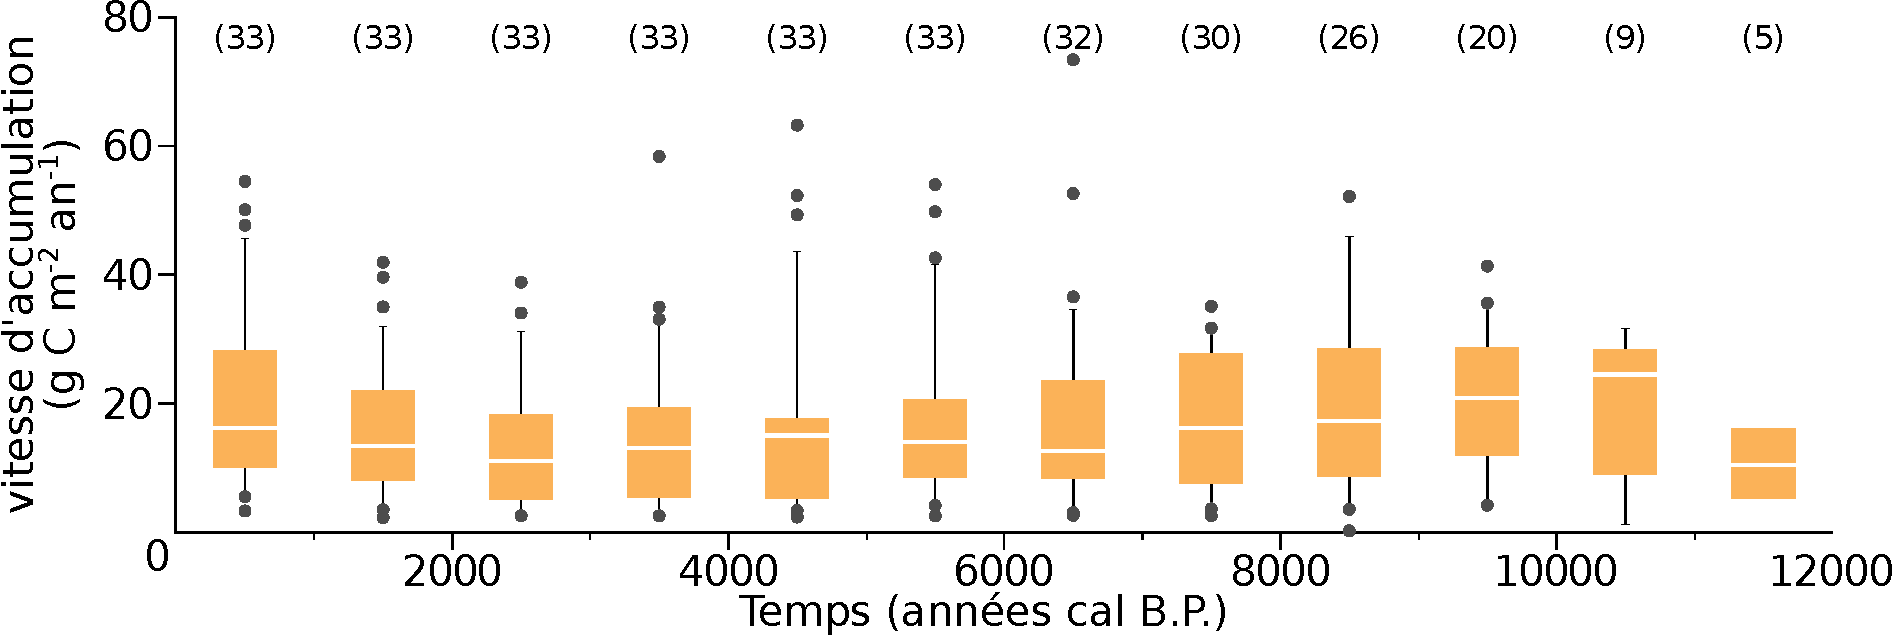
\includegraphics[width=\textwidth]{chap1/lorca}
\caption{Vitesse apparente d'accumulation du carbone à long terme durant l'Holocène. Les chiffres entre parenthèses représentent le nombre de mesures. Modifié d'après \citet{yu2009}}
\label{fig:lorca}
\end{figure}

\subsubsection{Bilans de carbone contemporains}

La seconde approche pour estimer le bilan de carbone d'écosystèmes est d'en estimer les flux actuels de carbone entrant et sortant.
Rappelons que les flux principaux dans le bilan de carbone d'une tourbière sont la PPB, la RE et le flux de \chh.
Cependant d'autres flux existent, notamment le flux de carbone organique dissout (COD), de carbone organique particulaire (COP), de carbone inorganique dissout (CID), de Composés Organiques Volatiles (COV), et de monoxyde de carbone (CO) \citep{chapin2006}.
Ils sont considérés comme négligeables, à l'exception du COD.
On définit ainsi le Bilan de Carbone Net de l'Écosystème (BCNE) comme :

\begin{equation}
%BCNE=\frac{dC}{dt}=\overbrace{PPB - Re}^{ENE}  - F_{COD} - F_{COP} - F_{CH_{4}} \textcolor{gray}{- F_{CID} - F_{COV} - F_{CO}}
BCNE=\frac{dC}{dt}=\overbrace{PPB - RE}^{ENE} - F_{CH_{4}} - F_{COD}
\label{bdc}
\end{equation}

Avec : 
\begin{itemize}
\item ENE : Échange Net de l'Écosystème
\item PPB : Production Primaire Brute
\item RE : Respiration de l'Écosystème
%\vspace*{.2cm}
\item F$_{CH_{4}}$ : Flux de Méthane
\item F$_{COD}$ : Flux de Carbone Organique Dissout
%\item F$_{COP}$ : Flux de Carbone Organique Particulaire
%\vspace*{.2cm}
%\item \textcolor{gray}{F$_{CID}$ : Flux de Carbone Inorganique Dissous}
%\item \textcolor{gray}{F$_{COV}$ : Flux de Composés Organique Volatils}
%\item \textcolor{gray}{F$_{CO}$ : Flux de Monoxyde de Carbone}
\end{itemize}

\begin{figure}
\centering
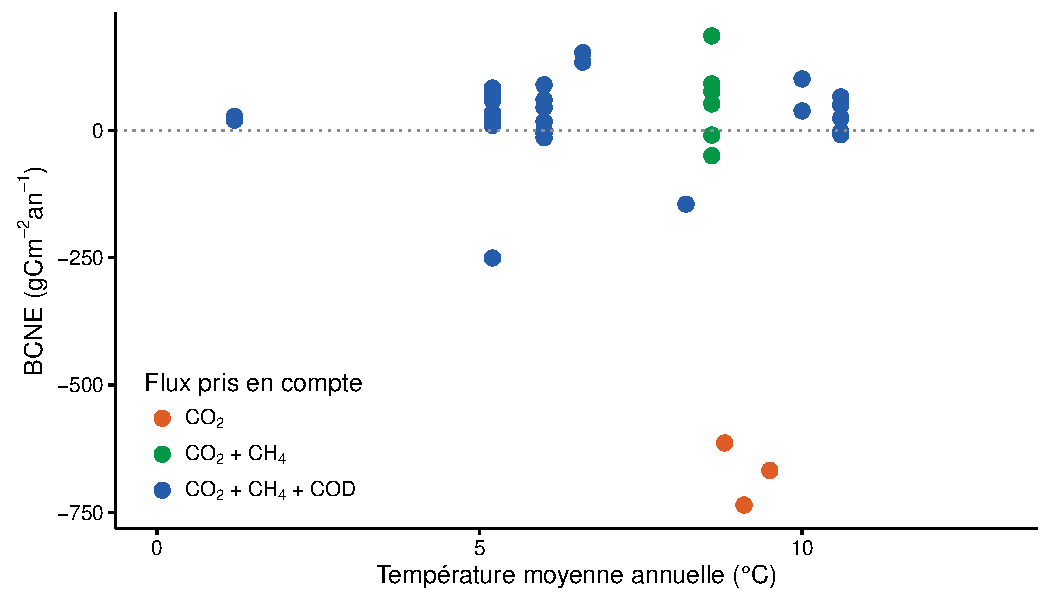
\includegraphics[width=\textwidth]{chap1/bib_necb}
\caption{Bilan de C dans différentes tourbières (en \si{\gcma}), en fonction de la température moyenne annuelle dans la littérature. Les couleur montrent quels flux sont pris en compte dans le bilan, la ligne de tirets sépare les écosystèmes stockant du carbone (au dessus) de ceux libérant du carbone (en dessous).}
\label{fig:bib_necb}
\end{figure}


Dans les tourbières, les flux de \coo sont généralement les plus importants puis les flux de \chh et/ou de COD et enfin les flux de COP \citep{worrall2009,koehler2011}.
Majoritairement réalisés dans les de haut-marais, les bilans de carbone rencontrés dans la littérature sont généralement compris entre 100 et \SI{-100}{\gcma} (Figure~\ref{fig:bib_necb}).
Si le stockage de carbone (NECB > 0) ne dépasse que peu de ces valeurs, le déstockage (NECB < 0) peut être beaucoup plus important avec des émissions de carbone de plus de \SI{500}{\gcma}.
Peu de bilans de carbone ont été faits dans les tourbières en dessous de \SI{50}{\degree} de latitude (le nord de la France approximativement).
Le comportement de ces tourbières les plus au sud reste peu connu par rapport à celles situées à des latitudes plus hautes (en Europe) ou dans des climats plus froids (au Canada).

\subsection{Méthodologies, mesures et estimation des flux}

\subsubsection{Méthode de mesure des flux de gaz}

Différentes techniques existent pour estimer les flux de gaz nécessaires pour le calcul des bilans de carbone.
Les méthodes les plus utilisées sont les techniques de chambres et les techniques micro-météorologiques.
%D'autres méthodes, moins souvent utilisées, existent comme l'utilisation du ratio C:N (Kirk2015)

De façon générale les méthodes de chambre consistent à placer une enceinte (ou chambre) sur une zone de l'écosystème dont où souhaite mesurer les flux.
Ces chambres peuvent être ouvertes : la mesure se fait lorsque le gaz à l'intérieur de la chambre est à l'équilibre avec celui à l'extérieur, ou fermées : le gaz à l'intérieur de la chambre n'est pas à l'équilibre avec celui à l'extérieur.
Elles peuvent également être dynamiques, lorsqu'un système de pompe permettant notamment de transporter le gaz jusqu'à l'analyseur est présent, ou statique si le système est sans flux artificiel.
Trois grandes techniques de chambre existent.
D'abord les chambres \textbf{dynamiques ouvertes} qui se basent sur un état d'équilibre et mesurent une différence de concentration d'un gaz dont une partie passe par la chambre et l'autre non. 
Cette méthode nécessite un système de pompe et donc l'existence d'un flux.
Ensuite les chambres \textbf{dynamiques fermées} qui mesurent l'évolution de la concentration du gaz au sein de la chambre à l'aide d'un système de pompe permettant l'envoi du gaz dans un analyseur externe.
Enfin les chambres \textbf{statiques fermées} qui mesurent également l'évolution de la concentration du gaz au sein de la chambre sans système de pompe.
Dans ce cas soit l'analyseur est présent dans la chambre, soit des prélèvements sont faits à intervalles réguliers puis analysés par la suite en chromatographie gazeuse.

Il faut noter que les dénominations anglaises de ces méthodes doivent faire l'objet d'une attention particulière.
\textit{Closed chamber} par exemple est parfois utilisé pour se référer à l'état ou non d'équilibre, comme défini dans ce document, mais parfois également pour désigner les méthodes de chambre sans système de flux ce qui peut prêter à confusion \citep{pumpanen2004}.
Souvent utilisées, les dénominations \textit{open}/\textit{closed} et \textit{dynamic}/\textit{static} sont décrites dans \citep{luo2006161}, une autre convention peut être rencontrée : \textit{flow-through}/\textit{non-flow-through} et \textit{steady state}/\textit{non-steady state} \citep{livingston1995}.

Ces différentes méthodes ont divers avantages et inconvénients : les systèmes sans circulation d'air sont généralement plus facile à transporter et à utiliser sur le terrain.
L'ensemble des méthodes de chambres fermées ont, par principe, une variation des concentrations en gaz qui, si elle est très importante, peut perturber le gradient de diffusion du gaz.
Malgré tout ces méthodes sont souvent utilisées car elles ont un coût modeste, et sont très versatiles ce qui permet leur utilisation dans de nombreuses situations.

D'autres méthodes plus globales existent comme les méthodes micro-météorologiques, basées sur l'étude des flux turbulents en analysant à haute fréquence la vitesse et la direction du vent.
Ces méthodes sont souvent appelées \textit{Eddy Covariance} ou \textit{Eddy Correlation}.
Elles sont beaucoup plus onéreuses et lourdes à mettre en place mais permettent une acquisition haute fréquence des flux de gaz.
Ces méthodes sont complémentaires aux mesures de chambre, car elles se font sur une zone plus grande que celles mesurées à l'aide de chambres.
La variabilité spatiale est donc intégrée dans la mesure, ce qui peut être un avantage comme un inconvénient.
La grande majorité des bilans pluriannuels sont faits à l'aide cette méthode.

\subsubsection{Estimation des flux}
Quand ils ne peuvent pas être mesurés avec une haute fréquence, que se soit à l'aide de tour Eddy-covariance ou de chambres automatiques, les flux sont estimés à partir de mesures ponctuelles.
La respiration est généralement estimée en utilisant la température que se soit celle de l'air \citep{bortoluzzi2006a} ou celle du sol à différentes profondeurs : \SI{-5}{\centi\metre} \citep{gorres2014,ballantyne2014}, \SI{-10}{\centi\metre} \cite{kim1992,zhu2015}.
Différentes équations reliant la respiration à la température sont utilisées \citep{fang2001}.
Le niveau de la nappe est parfois pris en compte \citep{strack2013,munir2015}, plus rarement la végétation \citep{bortoluzzi2006a,karki2015}.

L'estimation de la PPB est indirecte car très difficile à mesurer de façon directe à l'échelle d'un écosystème.
Elle est donc déduite à partir d'autres mesures :
Celles de l'ENE pour les méthodes micro-météorologiques qui utilisent l'ENE mesurée la nuit pour estimer la RE et en déduire la PPB.
Celles de l'ENE et de la RE pour les méthodes de chambre qui le permettent, ce qui permet là encore de déduire l'ENE.

Il existe donc une variabilité importante dans les équations utilisées, dans la nature et le nombre des facteurs pris en compte ainsi que dans la manière dont ils sont pris en compte.
